\documentclass[dvipsnames,12pt]{report} 
%\documentclass[12pt,twoside]{report}


%load any additional packages
\usepackage{amssymb}
\usepackage{amsmath}
\usepackage{graphicx}
\usepackage{multicol}
\usepackage{subfig}
\usepackage{lscape}
\usepackage{float}
\usepackage[document]{ragged2e}
\usepackage[colorinlistoftodos]{todonotes}
\usepackage{tikz}
\usepackage{dirtytalk}
\usetikzlibrary{shapes.geometric, arrows}
\usepackage[utf8]{inputenc}
\usepackage{multirow}
\usepackage{datetime}
\newdateformat{monthyeardate}{%
  \monthname[\THEMONTH], \THEYEAR}
\usepackage[english]{babel}
\usepackage{wrapfig}
\usepackage{rotating}
\usepackage{epstopdf}
\usepackage{algorithm}
\usepackage{algpseudocode}
\usepackage{pdfpages}
\usepackage{hyperref} 
\usepackage{enumitem}
\usepackage{subcaption}

%%%%%%%%%%%%%%%%%%%%%%%%%%%%%%%%%%%%%%%%%%%%%%%%%%%%%%%%%%%%%%%%%%%%%%%%%
\usepackage{fancyhdr}
\usepackage{color}
\usepackage{xcolor}
\pagestyle{fancy}
\fancyhead{}
% \fancyhead[LO,LE]{\scriptsize \mytitle}
%\fancyhead[RO,RE]{\leftmark}
%\fancyfoot{}
% \fancyfoot[CE,CO]{\footnotesize \thepage}
%\fancyfoot[LO,RE]{\footnotesize \leftmark}
%\fancyfoot[CO,CE]{\footnotesize}
%\fancyfoot[CE,CO]{Design of Low-Energy Level Shifter for Ultra Low-Voltage Emerging Applications}
%%%%%%%%%%%%%%%%%%%%%%%%%%%%%%%%%%%%%%%%%%%%%%%%%%%%%%%%%%%%%%%%%%%%%
%\usepackage[square,numbers]{natbib}
%\bibliographystyle{plainnat}
\bibliographystyle{IEEEtran}
%\usepackage[sectionbib]{chapterbib}
%\setcitestyle{square}

%%%%%%%%%%%%%%%%%%%%%%%%%%%%%%%%%%%%%%%%%%%%%%%%%%%%%%%%%%%%%%%%%%%%%%%%%
\setlength{\topmargin}{0.0in}
\setlength{\oddsidemargin}{0.33in}
\setlength{\evensidemargin}{-0.08in}
\setlength{\textheight}{8.5in}
\setlength{\textwidth}{6.0in}

\def\myprojectname{\textcolor{red}{Open-source Intelligence Data Mining System}}
\def\mytitle{Industry Internship Report \\on\\ \myprojectname}
\def\myname{Emmadi Sumith Kumar}
\def\mydegree{Specialization}
\def\mysupervisor{Dr Pradeep Kumar Roy}
\def\myrollno{UI20CS21}
\def\mydep{Computer Science and Engineering}
\def\mydegreedate{4\textsuperscript{th} Month, Year}

\setlength{\marginparwidth}{2cm}

\begin{document}
    \baselineskip=18pt plus pt
    \setcounter{secnumdepth}{3}
    \setcounter{tocdepth}{3}
    \pagenumbering{roman}
    %Front Matter
    \thispagestyle{empty}

\centering
    { \Large {\bfseries \textcolor{black}{{\mytitle}} \par}
\vspace{1.5\baselineskip}
    {\normalsize \textcolor{violet}{Submitted for the Partial Fulfillment of the}}\
    {\normalsize \textcolor{violet}{Requirements for the degree of Bachelor of Technology}}\par
\vspace{0.5\baselineskip}
    {\normalsize \textit{in} \par}
\vspace{0.5\baselineskip}
    {\large \bf \textcolor{violet}{\mydep}\par} 
\vspace{0.5\baselineskip}
    {\normalsize \textit{by} \par}
\vspace{0.5\baselineskip}
    {{\large {\bf \textcolor{ForestGreen}{\myname} \\ \textcolor{red}{Roll No.: \myrollno}}} \par}
%\vspace{-0.1\baselineskip}
%    {{\large {\bf \myrollno}} \par}
\vspace{1.1\baselineskip}
    {\textcolor{violet}{Under the guidance of}\par}
\vspace{0.5\baselineskip}
    {{\large \bf \textcolor{ForestGreen}{\mysupervisor} \par}
\vspace{0.5\baselineskip}
    {\begin{figure}[!h] 
	\centering
	
\includegraphics[width=30mm]{Formalities/IIIT_Surat_logo}\label{fig:figure2}
    \end{figure}
    }
%{\large \vspace*{1ex}
\vspace{1\baselineskip}
{\small \bf \textcolor{cyan}{DEPARTMENT OF \MakeUppercase{\mydep}} \par}
\vspace*{0.5ex}
{\small \bf July, 2024\par}
{\small \bf \textcolor{red}{\uppercase{Indian Institute of Information Technology Surat}-394190}}

    
    \phantomsection
    \addcontentsline{toc}{chapter}{Certificate}
    \thispagestyle{plain}

\begin{center}
{\Large {\textbf {\textcolor{red}{Indian Institute of Information Technology Surat}\\Computer Science and Engineering Department}}}
\end{center}

\vspace{1.25cm}
\justify


\begin{figure}[h]
    \centering
    
\includegraphics[width=30mm]{Formalities/IIIT_Surat_logo}\label{fig:figure}
\end{figure}

\begin{center}
{\Large {\bf \uppercase{Certificate}}}
\end{center}
\vspace{1.5cm}
\normalsize
\noindent This is to certify that candidate \textcolor{red}{\textbf{\myname}} bearing Roll No: \textcolor{red}{\textbf{\myrollno}} of B.TECH. IV, 8th Semester has successfully carried out the work on  ``\textcolor{red}{\textbf{\myprojectname}}" for the partial fulfillment of the degree of Bachelor of Technology (B.Tech.) in \textcolor{red}{\textbf{April, 2024}}.

\vspace{3\baselineskip}

\noindent Faculty Supervisor: \emph{Dr. Pradeep Kumar Roy}   \hfill Sign:\emph{…………………}\\
\vspace{1cm}

\noindent 1.  Examiner 1: \emph{ Dr. Pradeep Kumar Roy} \hfill Sign:\emph{…………………}\\
\vspace{0.3cm}

\noindent 2.  Examiner 2: \emph{ Mr. Vipul Kumar kania} \hfill Sign:\emph{…………………}\\
\vspace{0.3cm}

\noindent 3.  Examiner 3: \emph{ Ms. Jiby} T C \hfill Sign:\emph{…………………}\\
\vspace{0.3cm}

\begin{flushright} 

{\small \bf \textcolor{white}{}}\\
{\small \bf \textcolor{white}{}}\\
{\small (Seal of the Institute)} \\
\end{flushright}



% \begin{minipage}{0.45\textwidth}
% \noindent \\[1.5cm]
% {\small \bf Place: Shibpur} \\
% {\small \bf Date:}
% \end{minipage}

        
    \phantomsection
    \addcontentsline{toc}{chapter}{Declaration}
    \thispagestyle{plain}
\normalsize

\begin{center}
{\Large {\bf \uppercase{Declaration}}}
\end{center}

\vspace{\baselineskip}
\justify
\indent
This is to certify that \\
\noindent(i) This report comprises my original work towards the degree of Bachelor of Technology in Computer Science and Engineering at Indian Institute of Information Technology (IIIT) Surat and has not been submitted elsewhere for a degree,  \\
\noindent(ii) Due acknowledgement has been made in the text to all other material used.

\justify

\begin{minipage}{\textwidth}
\begin{flushright} 


{\small \bf \textcolor{white}{}}\\
{\small \bf \textcolor{white}{}}\\
{\small \bf Signature of Student} \\
{\small \bf (Emmadi Sumith Kumar)}\\[0.65cm]
\end{flushright}
\end{minipage}
\newpage
    
    \phantomsection
    \addcontentsline{toc}{chapter}{Acknowledgements}    
    \thispagestyle{plain}

\begin{center}
 \Large {\textbf \uppercase{Acknowledgement}}
\end{center}

\vspace{3\baselineskip}
\justify
I would like to express my heartfelt gratitude to all those who have helped me during my internship at \textbf{C-Trace Soft Solutions Private Limited} Company.

First, I am incredibly grateful to \textbf{Prof. Rajeev Shorey}, the Director of IIIT
Surat, for granting me the opportunity to undertake this internship.
His unwavering support and confidence in my abilities have been truly inspiring.
I also extend my heartfelt thanks to \textbf{Prof. J.S. Bhat}, the former Director of IIIT Surat, for his
support and guidance.

I would also like to thank my college supervisor, \textbf{Dr. Pradeep Kumar Roy}, for their constant support and encouragement during the internship.
Their insightful comments helped me to improve my work and gave me the confidence to take on new challenges.
I am deeply grateful to my company mentor,\textbf{ Mr. Venkata Rami Reddy Kasu}, who provided me with guidance, support, and valuable feedback throughout my internship.
Their expertise, patience, and kindness made a significant difference in my learning and professional growth.

I am grateful to the IIIT Surat and Training and Placement Cell of my college for providing me with the opportunity to pursue this internship.I feel privileged to have had the opportunity to work with such supportive and knowledgeable individuals, and I am grateful for their contribution to my professional development.


 
% \begin{flushright}
% \noindent
% \vspace{\baselineskip} \\
% .............................................\\
% \textbf{\myname} \\
% Place: IIEST Shibpur \\
% Date: \emph{……………}
% \end{flushright}
    
    \phantomsection
    \addcontentsline{toc}{chapter}{Abstract}
    \thispagestyle{plain}
\begin{center}
    \Large \textbf{\uppercase{Abstract}}
\end{center}

\vspace{3\baselineskip}

\vspace{1ex}
\justify

The aim of the \textbf{Open-source Intelligence Data Mining Application}  is to assist law enforcement agencies, such as police departments, in crime investigations by generating a report based on call data records (CDRs) and tower dump data. The software is designed to provide a rapid and efficient report, enabling investigators to identify suspects.
The primary objective of this software is to provide various information about individuals, including vehicle details, location data, IMEI numbers, phone numbers, PAN numbers, MNP details, IP information, etc. The software generates a PDF report containing all relevant information about the person.

The software is designed to be scalable, allowing for future enhancements and additions to accommodate evolving data collection requirements. Its success is dependent on technical infrastructure, legal compliance, user adoption, interoperability, and training and support for successful implementation.
The proposed software is already in use by several law enforcement agencies, This software has some pending features under development. It is continuously updated to meet the evolving needs of law enforcement agencies and to enhance its functionality and usefulness.
    
    
    
    \phantomsection
    \tableofcontents
    \protect

    \phantomsection
    \addcontentsline{toc}{chapter}{Symbols}
    \thispagestyle{plain}
\begin{raggedleft}
    \Huge \textbf{{List of Principal Symbols and Acronyms}}
\end{raggedleft}

\vspace{3\baselineskip}

\begin{enumerate}
    \item[] \makebox[3cm][l]{\fontsize{14}{16}\selectfont \textbf{VS}} \fontsize{14}{16}\selectfont \textbf{V}isual \textbf{S}tudio
    \item[] \makebox[3cm][l]{\fontsize{14}{16}\selectfont \textbf{OSINT}} \fontsize{14}{16}\selectfont \textbf{O}pen \textbf{S}ource \textbf{I}ntelligence
    \item[] \makebox[3cm][l]{\fontsize{14}{16}\selectfont \textbf{RC}} \fontsize{14}{16}\selectfont \textbf{R}egistration \textbf{C}ertificate
    \item[] \makebox[3cm][l]{\fontsize{14}{16}\selectfont \textbf{CRC}} \fontsize{14}{16}\selectfont \textbf{C}hasis to \textbf{R}egistration \textbf{C}ertificate
    \item[] \makebox[3cm][l]{\fontsize{14}{16}\selectfont \textbf{SMS}} \fontsize{14}{16}\selectfont \textbf{S}hort \textbf{M}essage \textbf{S}ervice
    \item[] \makebox[3cm][l]{\fontsize{14}{16}\selectfont \textbf{PAN}} \fontsize{14}{16}\selectfont \textbf{P}ermanent \textbf{A}ccount \textbf{N}umber
    \item[] \makebox[3cm][l]{\fontsize{14}{16}\selectfont \textbf{IP}} \fontsize{14}{16}\selectfont \textbf{I}nternet \textbf{P}rotocol
    \item[] \makebox[3cm][l]{\fontsize{14}{16}\selectfont \textbf{GPS}} \fontsize{14}{16}\selectfont \textbf{G}lobal \textbf{P}ositioning \textbf{S}ystem
    \item[] \makebox[3cm][l]{\fontsize{14}{16}\selectfont \textbf{IPL}} \fontsize{14}{16}\selectfont \textbf{I}nternet \textbf{P}rotocol \textbf{L}ogger
    \item[] \makebox[3cm][l]{\fontsize{14}{16}\selectfont \textbf{VN}} \fontsize{14}{16}\selectfont \textbf{V}irtual \textbf{N}umber
    \item[] \makebox[3cm][l]{\fontsize{14}{16}\selectfont \textbf{IMEI}} \fontsize{14}{16}\selectfont 
    \textbf{I}nternational \textbf{M}obile \textbf{E}quipment \textbf{I}dentity
    \item[] \makebox[3cm][l]{\fontsize{14}{16}\selectfont \textbf{PNR}} \fontsize{14}{16}\selectfont 
    \textbf{P}assenger \textbf{N}ame \textbf{R}ecord
    \item[] \makebox[3cm][l]{\fontsize{14}{16}\selectfont \textbf{IFSC}} \fontsize{14}{16}\selectfont 
    \textbf{I}ndian \textbf{F}inancial \textbf{S}ystem \textbf{C}ode
    \item[] \makebox[3cm][l]{\fontsize{14}{16}\selectfont \textbf{UPI}} \fontsize{14}{16}\selectfont 
    \textbf{U}nified \textbf{P}ayments \textbf{I}nterface
    \item[] \makebox[3cm][l]{\fontsize{14}{16}\selectfont \textbf{CC}} \fontsize{14}{16}\selectfont 
    \textbf{C}ourt \textbf{C}ase
    \item[] \makebox[3cm][l]{\fontsize{14}{16}\selectfont \textbf{BTS}} \fontsize{14}{16}\selectfont 
    \textbf{B}ase \textbf{T}ransceiver \textbf{S}tation
    \item[] \makebox[3cm][l]{\fontsize{14}{16}\selectfont \textbf{MNP}} \fontsize{14}{16}\selectfont 
    \textbf{M}obile \textbf{N}umber \textbf{P}ortability
    \item[] \makebox[3cm][l]{\fontsize{14}{16}\selectfont \textbf{AES}} \fontsize{14}{16}\selectfont 
    \textbf{A}dvanced \textbf{E}ncryption \textbf{S}tandard
    \item[] \makebox[3cm][l]{\fontsize{14}{16}\selectfont \textbf{VCS}} \fontsize{14}{16}\selectfont 
    \textbf{V}ersion \textbf{C}ontrol \textbf{S}ystem
    \item[] \makebox[3cm][l]{\fontsize{14}{16}\selectfont \textbf{DBMS}} \fontsize{14}{16}\selectfont 
    \textbf{D}atabase \textbf{M}anagement \textbf{S}ystem
    \item[] \makebox[3cm][l]{\fontsize{14}{16}\selectfont \textbf{IDE}} \fontsize{14}{16}\selectfont 
    \textbf{I}ntegrated \textbf{D}evelopment \textbf{E}nvironment
    \item[] \makebox[3cm][l]{\fontsize{14}{16}\selectfont \textbf{CI/CD}} \fontsize{14}{16}\selectfont 
    \textbf{C}ontinous \textbf{I}ntegration and \textbf{C}ontinous \textbf{D}eployment 
\end{enumerate}
    
    \phantomsection
    \addcontentsline{toc}{chapter}{List of Figures}
    \listoffigures
    % \listoftables

    \phantomsection
    \addcontentsline{toc}{chapter}{Format 3}
    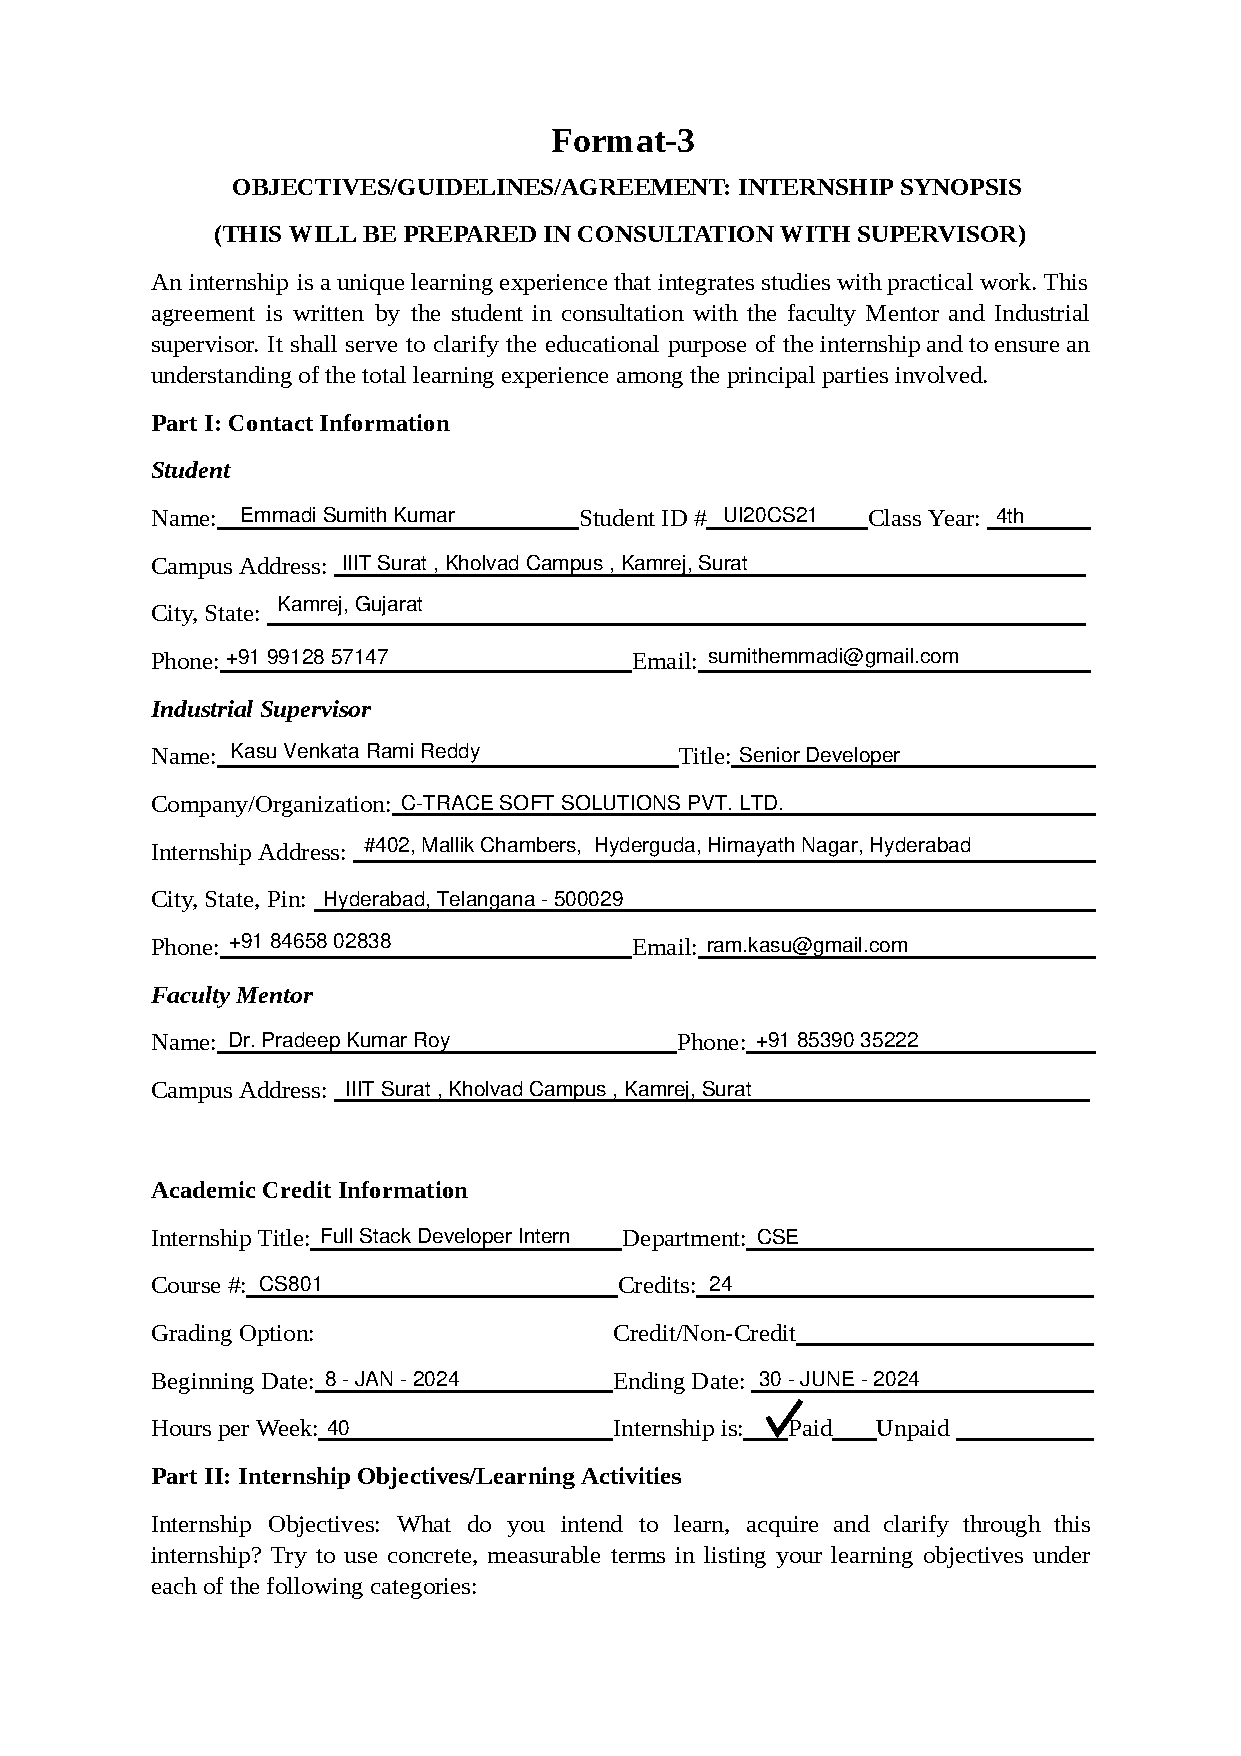
\includepdf[pages=-]{./UI20CS21_Format3.pdf}

    \phantomsection
    \addcontentsline{toc}{chapter}{Internship Completion Certificate}
    
\includepdf[pages=-]{./UI20CS21_INTERNSHIP_CERTIFICATE.pdf}

    %Main material
    \clearpage
    \pagenumbering{arabic}
    
    \chapter{Introduction}
\justify

The Open-source Intelligence Data Mining System (OSINT), as depicted in Figure 1.1, is an advanced software specifically designed to assist law enforcement agencies, such as the police department, in crime investigations by effectively analyzing call data records (CDRs) and tower dump data. It offers a comprehensive range of features crucial for conducting successful criminal investigations.

\begin{figure}
    \centering
    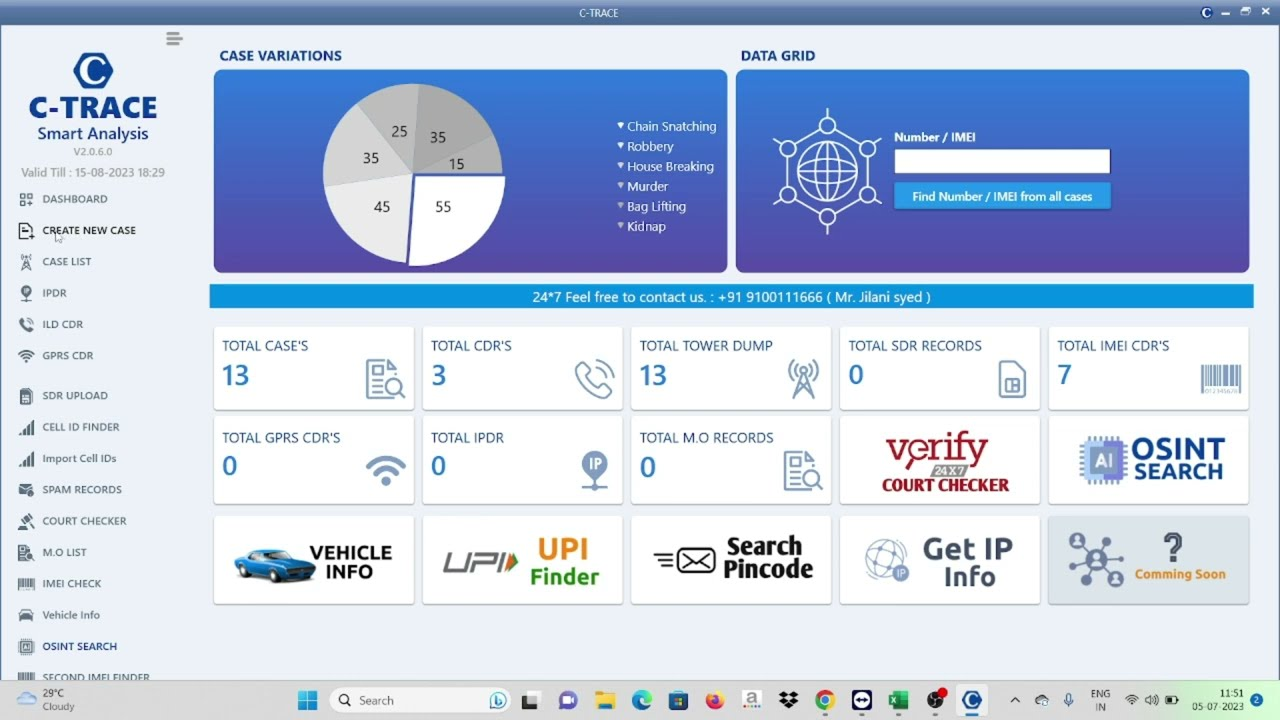
\includegraphics[width=1\linewidth]{Media/maxresdefault.jpg}
    \caption{C-Trace OSINT Software}
    \label{fig:C-Trace OSINT Software}
\end{figure}

The primary objective of this application is to provide law enforcement agencies with a rapid and efficient means of analyzing call data records (CDRs) and tower dump data. C-Trace OSINT software acts as a force multiplier, empowering investigators to make informed decisions and progress their investigations more effectively.

\section{What is OSINT Data Mining System ?}

The developed application is specifically designed for use by police departments only in solving crime cases by analyzing call data records (CDRs) and tower dump data. This software provides a detailed report on individuals using their phone number, IMEI number, PAN number, etc. It can extract tower data to identify all phone users within a specific tower, using azimuth ID. The report includes information such as the person's vehicle details, location data, IMEI numbers, phone numbers, PAN numbers, MNP details, IP information, and more. The software generates a PDF report that encompasses all relevant information about the individual.

\section{Features of OSINT Software}

The developed software provides a range of powerful search functionalities based query. Below are some of the key features offered:

\begin{enumerate}[label=\textbf{\roman*.}]
    \item \textbf{Vehicle information} : RC MH02ZX1234
    \item \textbf{IP Lookup} : IP 192.168.01.01
    \item \textbf{Pin code search} : PIN 524455
    \item \textbf{IMEI Search} : IMEI 45671234765823 \\
        You can Get Device Model details
    \item \textbf{PNR Search} : PNR 456789101 \\
        Check your train ticket status. Access passenger, seat, boarding, and destination info.
    \item \textbf{IFSC Search} : (e.g., "IFSC SBIN0062517" or "IFSC SBI ATTAPUR") \\
        Find bank details and IFSC codes for banks and cities.
    \item \textbf{UPI Search} : UPI 8465802838 \\
        Now, you can effortlessly retrieve UPI ID details by simply sending a UPI Mobile number. For instance, send UPI 8465802838
    \item \textbf{Court Case Search} : CC Name \\
        Now you can effortlessly track court cases of old offenders and suspects with our new Court Case Search feature. Simply send "CC Name" followed by the name of the individual, just like this: CC Prakash.
    \item \textbf{OSINT Search} : OSINT 9848012345 \\
        You can access names linked to phone numbers, UPI IDs, photos, social media accounts, and more.
    \item \textbf{Phone Number to Gas Connection search} : GAS 9848012345
    \item \textbf{Cell ID Search} : BTS 4044349032727 \\
        You can tower ID address and azimuth direction in Google Maps
    \item \textbf{MNP Lookup} : Network 9848012345 \\
        You can get mobile number portability details and Operator details
    \item \textbf{IMEI Last digit finder} : FULL IMEI 45231671101234 \\
        You can identify the last digit of an IMEI number.
\end{enumerate}

\section{Plugins Integrated with C-Trace OSINT Software}

This software is integrated with additional tools such as Verify 24x7 Court Checker, OSINT
Search, and Vehicle Information. These plugins enhance the software's capabilities and provide additional functionalities to law enforcement agencies.

\subsection{Verify 24x7 Court checker}

The Verify 24x7 Court checker is a third party tool that has large collection of court cases in India containing millions of records and updated on a daily basis. Given a name and address, our smart, proprietary algorithms retrieve matching cases in a few seconds.

This plugin allows users to verify the court case status of an individual by entering their name. This feature provides information on the individual's court cases, including the case number, court name, and case status. By utilizing this feature, law enforcement agencies can quickly verify the court status of suspects and offenders, aiding in their investigations and intelligence gathering.

\subsection{OSINT Search}

OSINT Search is a feature that allows users to gather publicly available information about individuals, including personal and public details, to aid in investigations. By utilizing OSINT (Open-Source Intelligence) techniques, this feature helps retrieve relevant information about the suspect, such as their personal background, social
media activity, online presence, and other publicly accessible data. This
comprehensive search capability assists law enforcement agencies and investigators in building a more complete profile of the culprit, aiding in the investigation process.

\subsection{Vehicle Information}

Vehicle Information is a feature that allows users to obtain details about a specific vehicle using its registration number. By inputting the vehicle number into the system, investigators can retrieve information such as the make, model, year of manufacture, color, and ownership details of the vehicle associated with that registration number. This feature is valuable in investigations as it helps identify and track vehicles linked to criminal activities, providing important leads for law enforcement agencies and helping them in their pursuit of the culprits.

\section*{The rest of the Report is organized as follows:}
\begin{itemize}
    \item \textbf{Chapter 2:} Tools and Technologies
    \item \textbf{Chapter 3:} Proposed Systems
    \item \textbf{Chapter 4:} Design
    \item \textbf{Chapter 5:} Implementation
    \item \textbf{Chapter 6:} Testing and Experimental Results
    \item \textbf{Chapter 7:} Conclusion and Future Scope
\end{itemize}

\newpage




    \chapter{Tools and Technologies}

\justify
{\myprojectname} encompasses a wide range of tools and technologies that facilitate the creation, deployment, and maintenance of applications. From integrated development environments (IDEs) for coding to version control systems (VCS) for collaboration, programming languages, frameworks, database management systems (DBMS), containerization tools, continuous integration/continuous deployment (CI/CD) pipelines, cloud platforms, testing tools, API development tools, code editors, project management platforms, security tools, and monitoring/logging solutions, the software development landscape is rich and diverse, catering to various aspects of the development lifecycle.
\section{Tools}
\justify

React Native is a popular open-source framework developed by Facebook for building mobile applications using JavaScript and React. It allows developers to create native mobile apps for both iOS and Android platforms using a single codebase. However, since you specifically asked about Android apps, I'll focus on that aspect.

% \begin{figure}
%   \centering
%   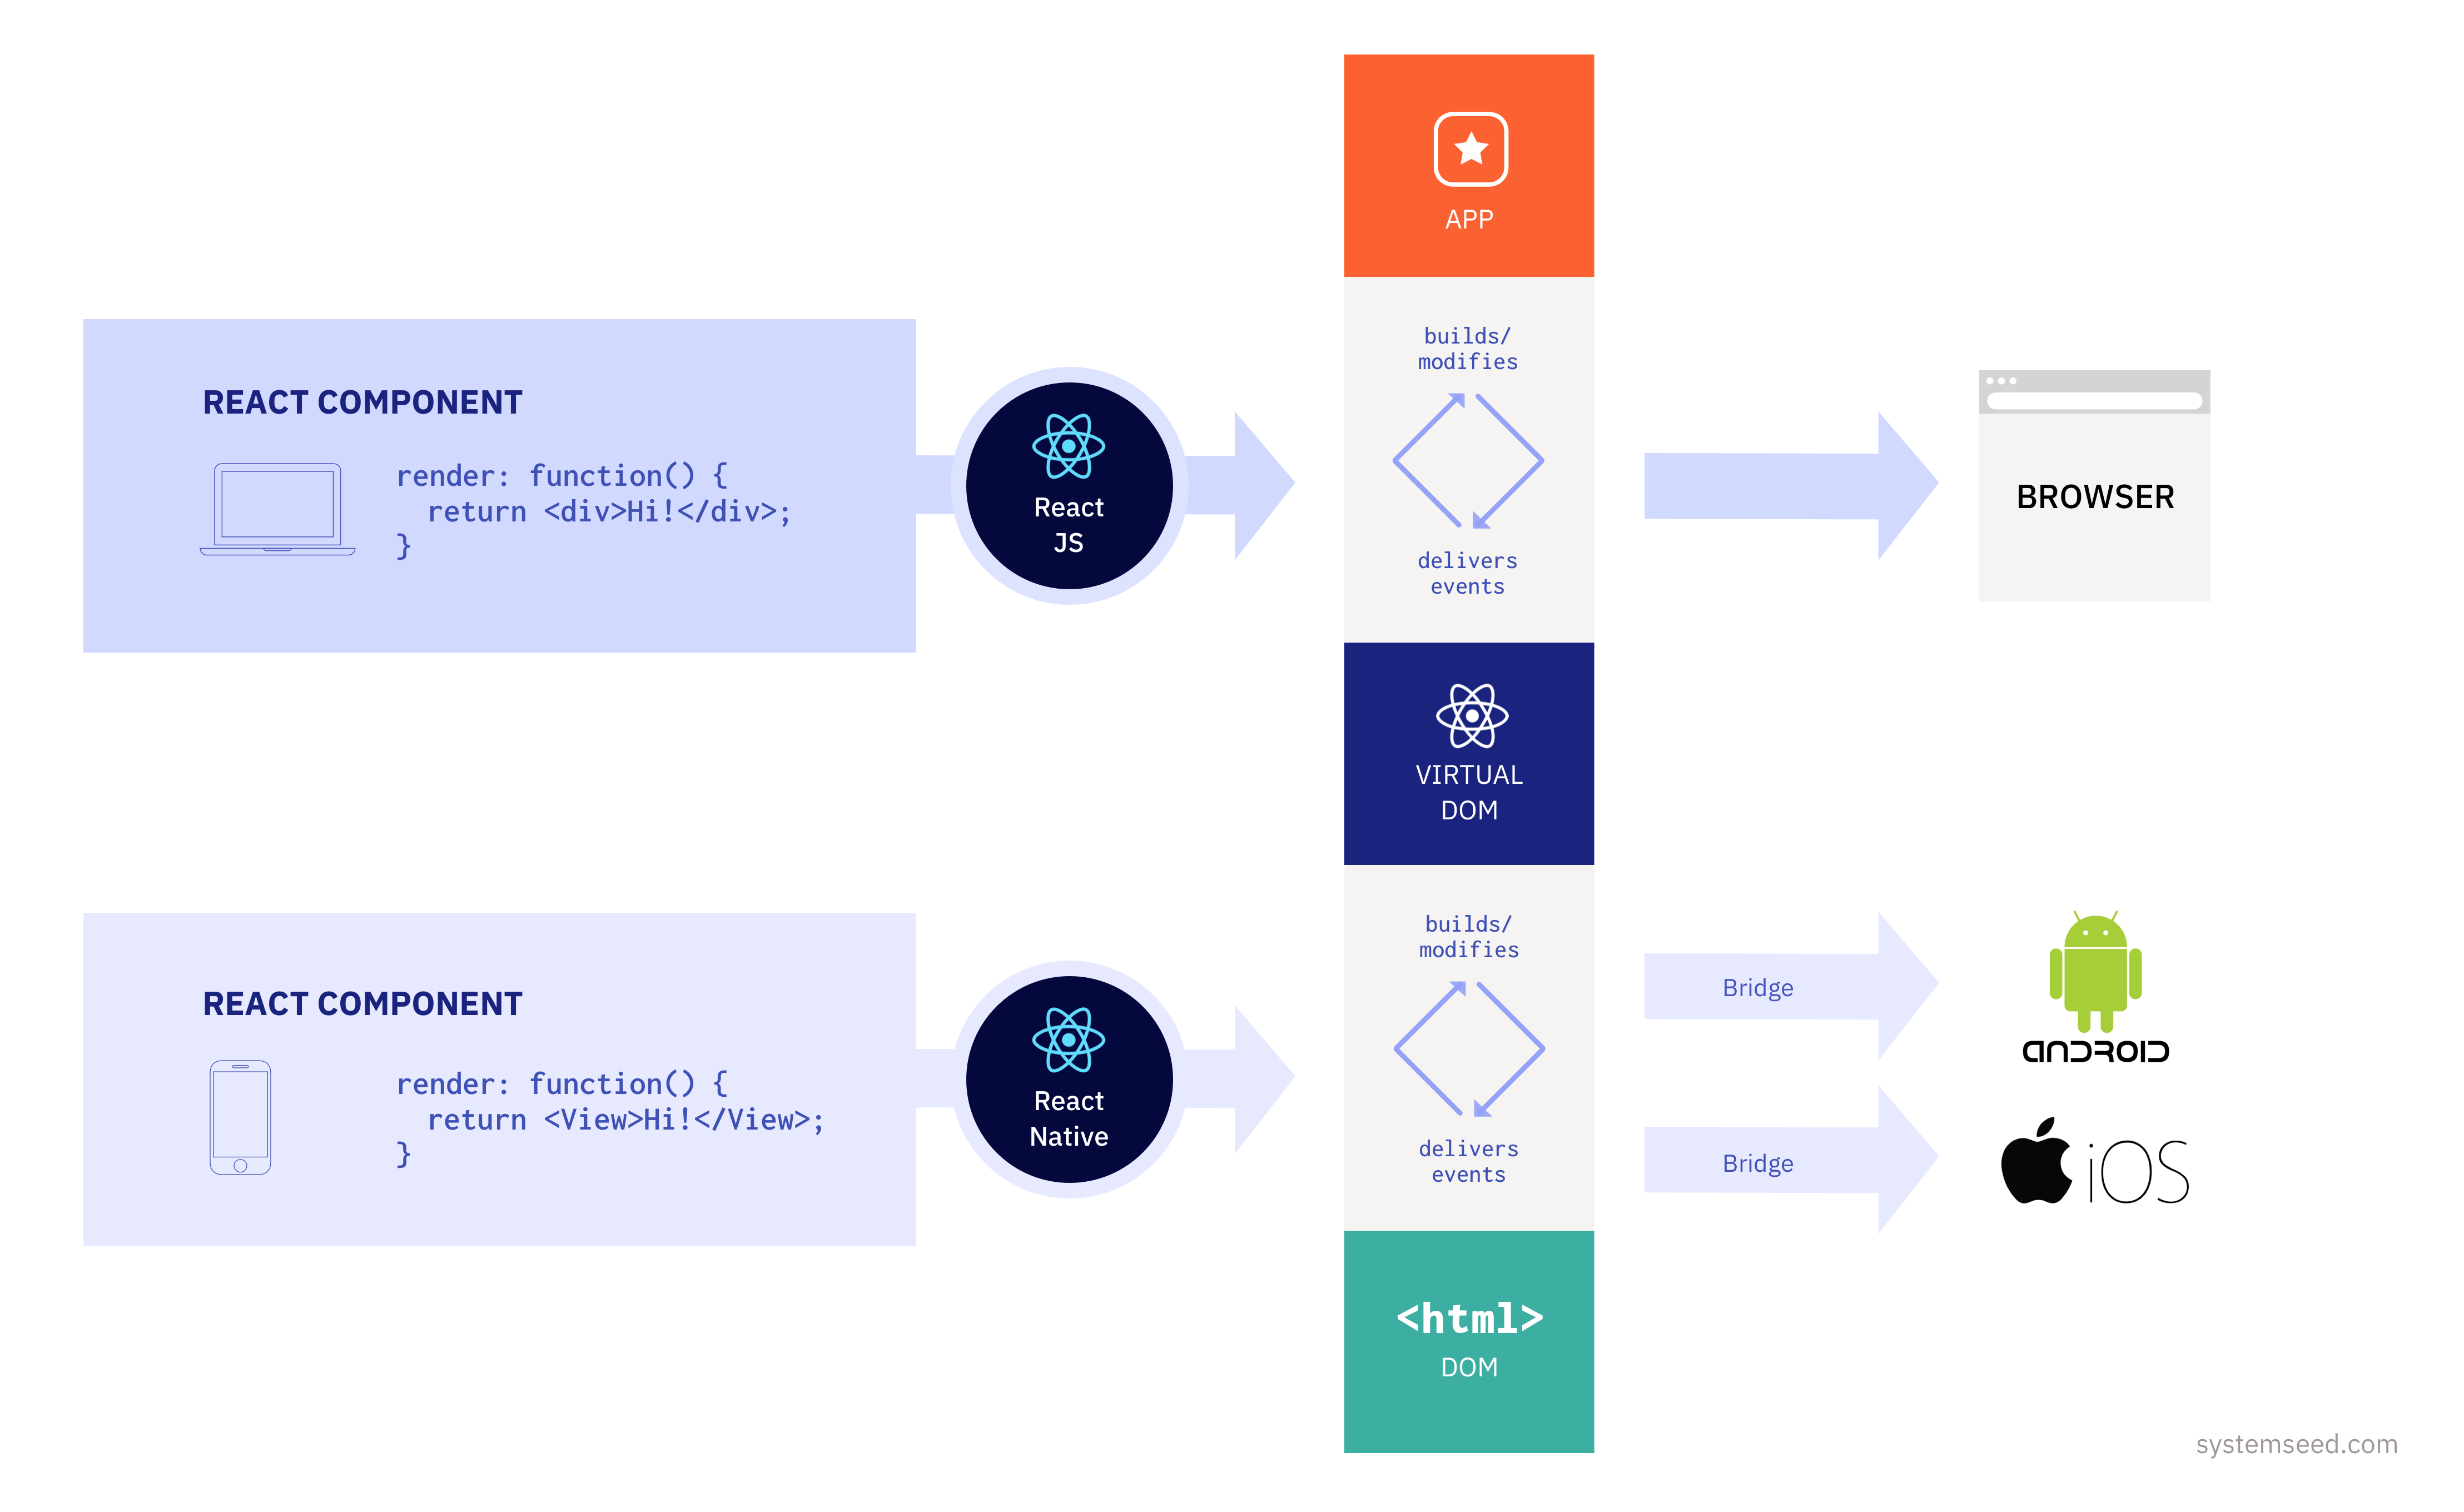
\includegraphics[width=0.90\linewidth]{Media/react-diagram_3.png}
%   \caption{React Native}
%   \label{fig:React Native}
% \end{figure}

\begin{enumerate}
  \item \textbf{Visual Studio Code}: Used Visual Studio Code to design the OSINT Software and also used 
  
  \item \textbf{Flipper}: One of the primary advantages of React Native is its ability to support cross-platform development. Developers can write code once and deploy it on both iOS and Android platforms, saving time and effort compared to building separate native apps for each platform.
  
  \item \textbf{React Native Debugger}: React Native allows developers to create native components using JavaScript, which are then rendered using native APIs. This approach enables the development of high-performance apps with a native look and feel, as the components are rendered using the underlying platform's UI elements.
  
  \item \textbf{HTTPie}: React Native includes a feature called hot reloading, which allows developers to see the changes they make to the code in real-time without restarting the app. This can significantly speed up the development process and improve productivity.
  
  \item \textbf{Android Studio}: React Native provides access to native modules and APIs through a bridge mechanism. This means developers can integrate platform-specific functionalities such as camera, geolocation, push notifications, etc., into their apps seamlessly.
  
  \item \textbf{Android Emulator}: React Native has a vibrant ecosystem of third-party libraries, plugins, and community-contributed components that developers can leverage to add additional features and functionalities to their apps.
  
  \item \textbf{Git}: While React Native offers good performance out of the box, developers can further optimize their apps for performance by implementing best practices, using efficient code patterns, and utilizing tools like performance profiling and debugging tools provided by React Native.
  
  \item \textbf{Chromium Browser}: React Native supports various testing and debugging tools, including Jest for unit testing, React Native Debugger for debugging, and tools like Flipper for inspecting app performance and behavior. 

  \item \textbf{DBeaver}: React Native supports various testing and debugging tools, including Jest for unit testing, React Native Debugger for debugging, and tools like Flipper for inspecting app performance and behavior. 

  \item \textbf{Nginx}: React Native supports various testing and debugging tools, including Jest for unit testing, React Native Debugger for debugging, and tools like Flipper for inspecting app performance and behavior. 

  \item \textbf{Puppeteer}: React Native supports various testing and debugging tools, including Jest for unit testing, React Native Debugger for debugging, and tools like Flipper for inspecting app performance and behavior. 
  
  \begin{figure}
    \centering
    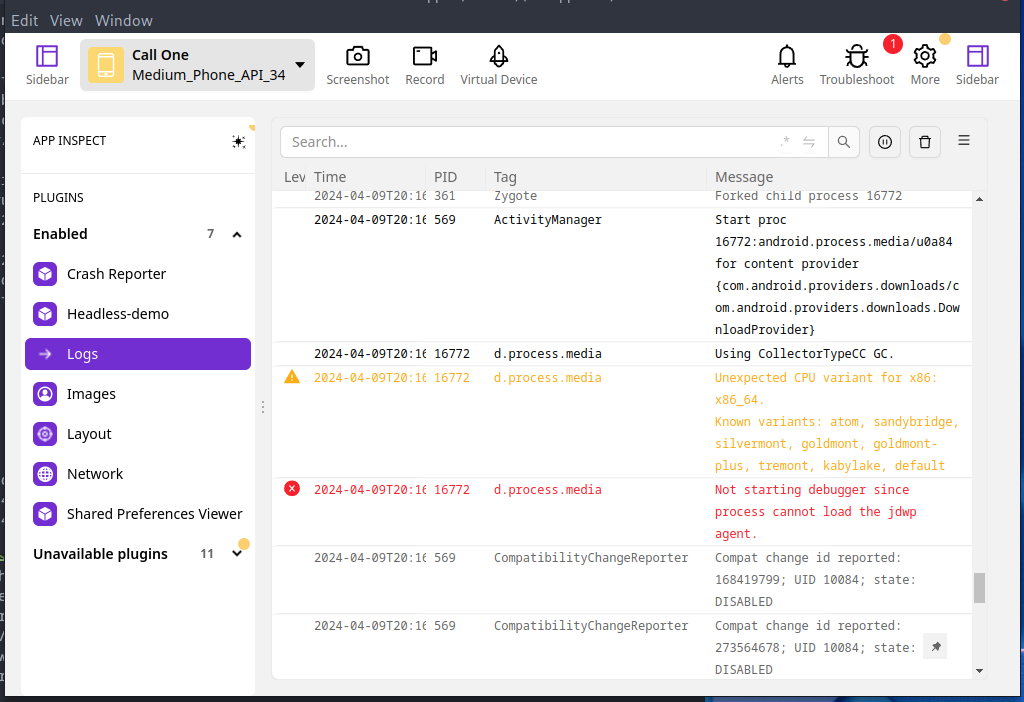
\includegraphics[width=1\linewidth]{Media//Chapter 6/flipper.png}
    \caption{Flipper Debugging}
    \label{fig:Flipper Debugging}
  \end{figure}
\end{enumerate}


\section{Technologies}
\justify

React Native is a popular open-source framework developed by Facebook for building mobile applications using JavaScript and React. It allows developers to create native mobile apps for both iOS and Android platforms using a single codebase. However, since you specifically asked about Android apps, I'll focus on that aspect.

% \begin{figure}
%   \centering
%   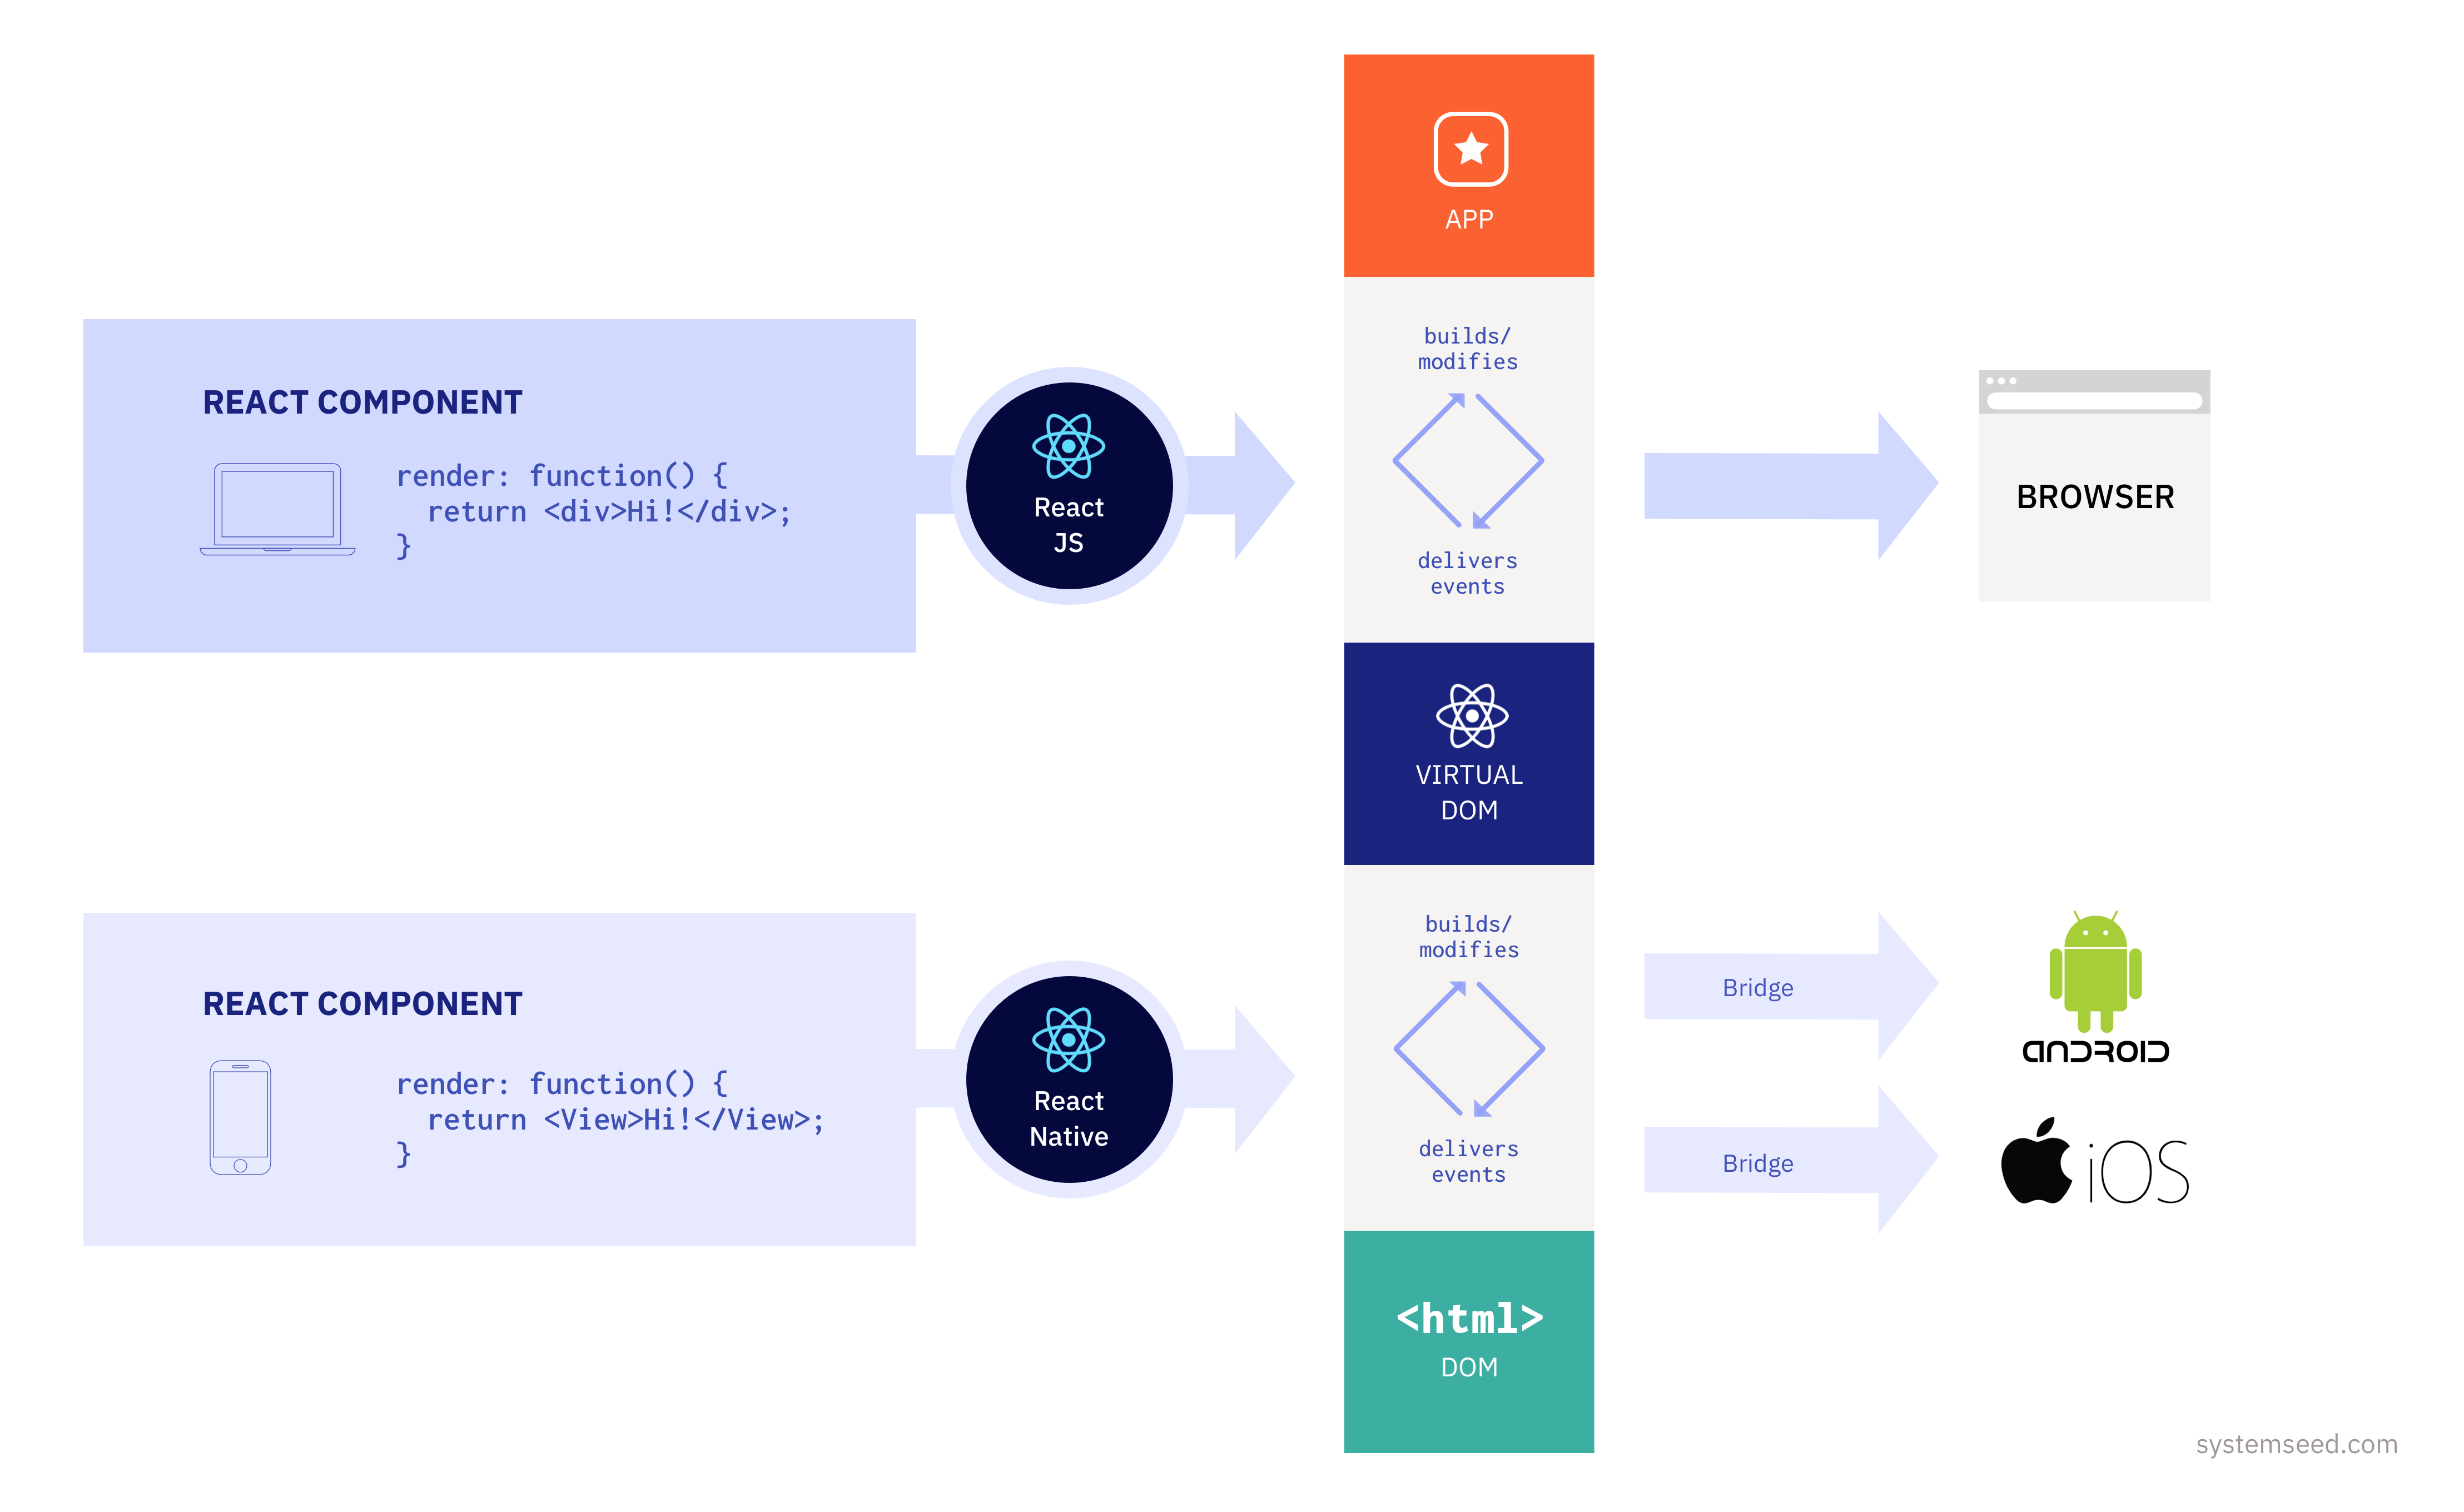
\includegraphics[width=0.90\linewidth]{Media/react-diagram_3.png}
%   \caption{React Native}
%   \label{fig:React Native}
% \end{figure}

\begin{enumerate}
  \item \textbf{React Native}: React Native utilizes JavaScript as the programming language and React as the JavaScript library for building user interfaces. This combination enables developers to write code in a familiar language and leverage React's component-based architecture for UI development.
  
  \item \textbf{Kotlin}: One of the primary advantages of React Native is its ability to support cross-platform development. Developers can write code once and deploy it on both iOS and Android platforms, saving time and effort compared to building separate native apps for each platform.
  
  \item \textbf{JavaScript}: React Native allows developers to create native components using JavaScript, which are then rendered using native APIs. This approach enables the development of high-performance apps with a native look and feel, as the components are rendered using the underlying platform's UI elements.
  
  \item \textbf{TypeScript}: React Native includes a feature called hot reloading, which allows developers to see the changes they make to the code in real-time without restarting the app. This can significantly speed up the development process and improve productivity.
  
  \item \textbf{Express.js}: React Native provides access to native modules and APIs through a bridge mechanism. This means developers can integrate platform-specific functionalities such as camera, geolocation, push notifications, etc., into their apps seamlessly.
  
  \item \textbf{Node.js}: React Native has a vibrant ecosystem of third-party libraries, plugins, and community-contributed components that developers can leverage to add additional features and functionalities to their apps.
  
  \item \textbf{Crypto-js}: While React Native offers good performance out of the box, developers can further optimize their apps for performance by implementing best practices, using efficient code patterns, and utilizing tools like performance profiling and debugging tools provided by React Native.

  \item \textbf{PostgreSQL}: While React Native offers good performance out of the box, developers can further optimize their apps for performance by implementing best practices, using efficient code patterns, and utilizing tools like performance profiling and debugging tools provided by React Native.
 
  \item \textbf{React Native Firebase}: React Native supports various testing and debugging tools, including Jest for unit testing, React Native Debugger for debugging, and tools like Flipper for inspecting app performance and behavior. 
  
  \item \textbf{JSON Web Tokens (JWT)}: While React Native offers good performance out of the box, developers can further optimize their apps for performance by implementing best practices, using efficient code patterns, and utilizing tools like performance profiling and debugging tools provided by React Native.
  
  \item \textbf{PDFKit}: While React Native offers good performance out of the box, developers can further optimize their apps for performance by implementing best practices, using efficient code patterns, and utilizing tools like performance profiling and debugging tools provided by React Native.
  
  \item \textbf{Baileys (WhatsApp Client)}: While React Native offers good performance out of the box, developers can further optimize their apps for performance by implementing best practices, using efficient code patterns, and utilizing tools like performance profiling and debugging tools provided by React Native.
  

  \begin{figure}
    \centering
    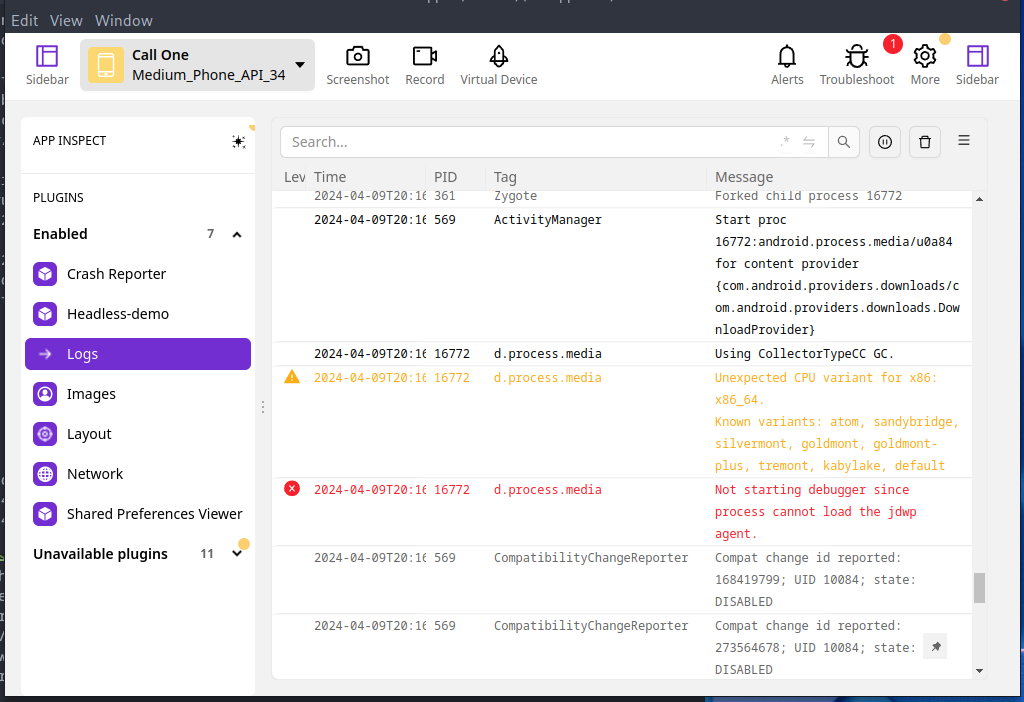
\includegraphics[width=1\linewidth]{Media//Chapter 6/flipper.png}
    \caption{Flipper Debugging}
    \label{fig:Flipper Debugging Tool}
  \end{figure}
\end{enumerate}


\section{Kotlin}

In our Android application development, Kotlin played a crucial role in implementing various functionalities to enhance user experience and ensure data security. This section discusses how Kotlin was used for phone call modules, phone state receiver, and AES encryption for transmitting data to the backend.

\subsection{Phone Call Modules}

Kotlin was utilized to create phone call modules within our app, allowing users to make phone calls directly from the application. This feature streamlined the communication process and provided a seamless experience for users. Key aspects of the phone call modules include:

\begin{enumerate}
  \item Initiating outgoing calls from within the app.
  \item Integrating call management functionalities, such as call duration tracking and call logs.
  \item Ensuring compatibility with different Android devices and versions.
\end{enumerate}

Kotlin's concise syntax and robust features enabled us to develop efficient phone call modules that integrated seamlessly with the app's user interface and functionality.

\subsection{Phone State Receiver}

A phone state receiver implemented in Kotlin was used to detect various call events, including incoming calls, outgoing calls, and ongoing calls. This receiver played a crucial role in managing call-related actions within the app. Key functionalities of the phone state receiver include:

\begin{enumerate}
  \item Detecting incoming calls and displaying caller information.
  \item Monitoring call status changes, such as call answered, call ended, etc.
  \item Handling call-related actions, such as rejecting incoming calls or pausing ongoing calls.
\end{enumerate}

Kotlin's event handling capabilities and compatibility with Android's telephony APIs made it a suitable choice for implementing the phone state receiver.

\subsection{AES Encryption for Data Transmission}

To ensure data security during data transmission to the backend server, AES (Advanced Encryption Standard) encryption was implemented using Kotlin. This encryption technique was applied to encrypt user data and queries before transmitting them over the network. Key aspects of AES encryption integration include:

\begin{enumerate}
  \item Encrypting sensitive user information, such as credentials and personal data, to protect against unauthorized access.
  \item Encrypting data queries to maintain confidentiality and integrity during transmission.
  \item Implementing secure key management practices to generate and store encryption keys securely.
\end{enumerate}


\section{PostgreSQL}

In our application's backend infrastructure, we leveraged PostgreSQL as the database management system for storing user information securely and efficiently. This section outlines how PostgreSQL was utilized to store user data, including the storage of JSON objects in an array format and optimizing queries for fast retrieval.

We designed a PostgreSQL database schema to accommodate various types of user information, such as user profiles, preferences, transactions, and more. The database tables were structured to efficiently store and manage user data while ensuring data integrity and scalability.

For storing JSON objects, we utilized PostgreSQL's native support for JSON data types. Specifically, we stored JSON objects in arrays within PostgreSQL tables, allowing us to organize and manage structured data effectively.


\begin{enumerate}
  \item \textbf{Structured Data Storage}: JSON arrays provided a structured format for storing related data elements, such as an array of user preferences or a list of user transactions.
  
  \item \textbf{Flexible Data Retrieval}: PostgreSQL's JSON functions and operators allowed us to query and manipulate JSON data within arrays, facilitating flexible data retrieval and processing.
  
  \item \textbf{Reduced Data Redundancy}: Storing JSON objects in arrays minimized data redundancy by grouping related data elements together, optimizing storage space and database performance.
  
  \item \textbf{Indexing}: We created appropriate indexes on database columns used in frequent queries, such as user IDs, to accelerate data retrieval operations.
  
  \item \textbf{Query Optimization}: We optimized SQL queries by utilizing PostgreSQL's query planner and execution engine, ensuring optimal query performance and resource utilization.
  
  \item \textbf{Caching}: Where applicable, we implemented caching mechanisms at the application layer to reduce database load and improve response times for frequently accessed data.
\end{enumerate}

To ensure fast and efficient retrieval of user information from the PostgreSQL database, we optimized database queries using various techniques, including:


By combining efficient database schema design, storage of JSON objects in arrays, and query optimization techniques, we achieved fast and reliable data retrieval capabilities from the PostgreSQL database, enhancing overall application performance and user experience.



\section{React Native Firebase}

In our mobile application development using React Native, we leveraged React Native Firebase for implementing Google SignIn functionality. This section outlines how React Native Firebase facilitated seamless integration with Google SignIn and enhanced user authentication capabilities.

\subsection{Integration with React Native Firebase}

React Native Firebase provides a comprehensive set of Firebase services for React Native apps, including authentication services like Google SignIn. By integrating React Native Firebase into our project, we gained access to Firebase's authentication APIs, simplifying the implementation of Google SignIn.

\section{Flipper}

Flipper is a powerful debugging and development tool created by Facebook for mobile app developers. It provides a suite of features and capabilities that streamline the debugging and testing process, enhancing productivity and improving the overall quality of mobile applications.

\subsection{Key Features of Flipper}

\begin{enumerate}
  \item \textbf{UI Inspector}: Flipper allows developers to inspect and debug the user interface (UI) of their mobile apps in real-time. Developers can view the layout hierarchy, inspect UI elements, and identify issues or inconsistencies easily.
  
  \item \textbf{Network Inspector}: With Flipper's network inspector, developers can monitor network requests made by their app, view request and response details, analyze network performance, and debug network-related issues efficiently.
  
  \item \textbf{Database Viewer}: Flipper provides a database viewer tool that allows developers to inspect and interact with local databases used by their mobile apps. This feature is particularly useful for debugging data storage and retrieval functionalities.
  
  \item \textbf{Performance Profiling}: Flipper offers performance profiling tools that enable developers to analyze app performance metrics, identify performance bottlenecks, and optimize app performance for better user experience.
  
  \item \textbf{Crash Reporting}: Flipper integrates with crash reporting services, providing developers with insights into app crashes, error logs, and crash analytics. This helps in identifying and resolving critical issues that impact app stability.
\end{enumerate}


\section{JSON Web Tokens (JWT)}

JSON Web Tokens (JWT) are a popular method for managing sessions and authentication in web and mobile applications, including Android apps. In our Android app development, we leveraged JWT for secure and efficient session management. This section outlines how JWT tokens were utilized to manage user sessions in our Android app.

\subsection{JWT Token Generation}

When a user successfully logs in or authenticates in our Android app, a JWT token is generated by the backend server. This JWT token contains encoded user information, such as user ID, roles, and expiration time. The JWT token is then securely stored on the client-side, typically in the app's local storage or shared preferences.

\subsection{Token-Based Authentication}

For subsequent API requests or operations requiring authentication, the JWT token is sent along with the request headers. The backend server verifies the JWT token's authenticity and validity before processing the request. This token-based authentication mechanism eliminates the need for storing session information on the server-side, reducing server load and improving scalability.

\subsection{Token Expiration and Refresh}

JWT tokens have an expiration time set during token generation. When a JWT token expires, the client app can request a new token using a refresh token mechanism. The refresh token is a separate token with a longer expiration time, used to obtain a new JWT token without requiring the user to log in again. This ensures seamless and continuous session management in the app.


\section{Express.js}
In our application's backend development, we utilized Express.js, a popular Node.js framework, to build robust and scalable APIs for handling various functionalities. This section delves into how Express.js was used along with TypeScript for creating APIs, integrating with Next.js, and implementing encryption for secure data handling.

\subsection{APIs for User Contacts and Call Logs}

Using Express.js, we created RESTful APIs to manage user contacts and call logs. These APIs allowed users to:

\begin{enumerate}
  \item Store and retrieve user contacts, including name, phone number, and additional details.
  \item Log incoming and outgoing calls, along with call duration, timestamps, and caller/callee information.
  \item Perform CRUD operations on contacts and call logs, enabling efficient data management.
\end{enumerate}

Express.js's middleware and routing capabilities facilitated the implementation of these APIs, providing a structured and organized approach to backend development.

\subsection{AES Encryption for Secure Query Handling}

To enhance data security, we implemented AES (Advanced Encryption Standard) encryption for handling encrypted queries, especially when searching for a phone number. Key aspects of AES encryption integration include:

\begin{enumerate}
  \item Encrypting user queries containing sensitive information, such as phone numbers, before processing them in the backend.
  \item Decryption of encrypted queries using the AES decryption algorithm to retrieve relevant data securely.
  \item Utilizing secure key management practices to generate and manage encryption keys for AES encryption and decryption.
\end{enumerate}

By incorporating AES encryption, we ensured that user data and queries remained secure and protected against unauthorized access or interception.

\subsection{Integration with Next.js as a Custom Server}

Express.js was integrated as a custom server with Next.js, a React framework for frontend development, to run both backend and frontend on the same server. This integration provided several benefits:

\begin{enumerate}
  \item Simplified deployment and hosting, with a single server instance serving both backend APIs and frontend UI components.
  \item Improved performance and reduced latency due to server-side rendering (SSR) capabilities of Next.js.
  \item Seamless communication between backend APIs and frontend components, enhancing user experience and application responsiveness.
\end{enumerate}

Express.js and Next.js integration offered a cohesive development environment, streamlining the development and deployment process of our application.

\subsection{TypeScript}

For enhanced code quality and maintainability, we leveraged TypeScript with Express.js. TypeScript provided:

\begin{enumerate}
  \item Static typing and type checking, preventing type-related errors and improving code reliability.
  \item Better code documentation and readability with explicit type definitions for variables, functions, and API contracts.
  \item Improved development experience with features like code completion, refactoring tools, and type inference.
\end{enumerate}

TypeScript's integration with Express.js facilitated a more robust and structured backend codebase, enhancing code quality and developer productivity.


\section{Puppeteer}

In our software, we employed Puppeteer, a Node.js library, to scrape images associated with a phone number from Google Contacts. This section details how Puppeteer was used for this purpose and the steps involved in the scraping process. we installed Puppeteer as a Node.js dependency in our project using npm or yarn. Puppeteer provides a high-level API for controlling headless Chrome or Chromium browsers, making it suitable for automating web scraping tasks.


\section{PDFKit}

In our information gathering and analysis process, we utilized PDFKit, a Node.js library, to create a comprehensive OSINT (Open-Source Intelligence) report. This note outlines how PDFKit was employed to generate professional and structured reports based on gathered intelligence.

% \begin{figure}
%     \centering
%     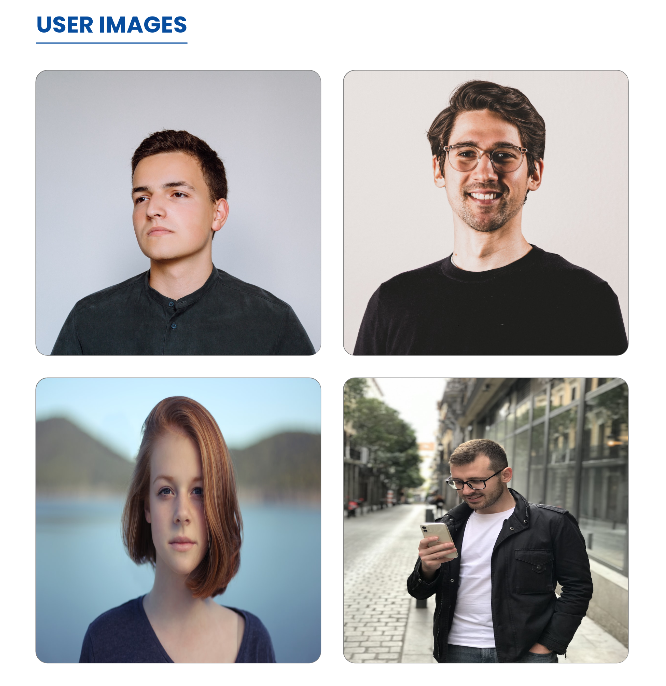
\includegraphics[width=1\linewidth]{Media//Chapter 2/image.png}
%     \caption{User Image From OSINT Report}
%     \label{fig:User Image From OSINT Report}
% \end{figure}
  
\subsection{Integration of PDFKit}

PDFKit was seamlessly integrated into our Node.js application as a dependency using npm or yarn. This library provides a straightforward and efficient API for programmatically generating PDF documents, making it ideal for creating detailed reports.

\section{Baileys (WhatsApp Client)}

Baileys is a  WhatsApp client library designed in Node.js. It provides a simple yet powerful interface for interacting with WhatsApp's API, allowing developers to access user information such as name, photo, and online status.

\subsection{Features}

\begin{enumerate}
  \item \textbf{User Information Retrieval}: Baileys allows developers to retrieve essential user details from WhatsApp, including the user's name, profile photo, and online status. This information can be useful for building personalized messaging experiences and user management features.
  
  \item \textbf{Integration with Node.js}: Baileys seamlessly integrates with Node.js applications, making it easy for developers to incorporate WhatsApp functionalities into their projects. This integration enables developers to create chatbots, automate messaging tasks, and implement custom user interactions.

\end{enumerate}





    
\chapter{Proposed System}\label{ch:proposed-system}
\justify

This chapter provides a detailed overview of the Open-source Intelligence Data Mining System.
The project main aim is to collect Open Source and Internet Exposed information for law enforcement purposes, along with the objectives, assumptions, dependencies, and system requirements essential for its implementation.

\section{Objectives}\label{sec:objectives}

The primary objective of this application is to provide law enforcement agencies with a rapid and efficient means of analyzing call data records (CDRs) and tower dump data.
C-Trace OSINT software acts as a force multiplier, empowering investigators to make informed decisions and progress their investigations more effectively.
Specifically, the objectives are as follows:

\begin{enumerate}[label=\roman*.]
    \item To collect various types of information from individuals, including:
    \begin{itemize}
        \item Vehicle details
        \item Location data
        \item IMEI numbers
        \item Phone numbers
        \item PAN numbers
        \item MNP details
        \item IP information
        \item Court cases
        \item PNR information and more
    \end{itemize}
    \item To develop a caller ID app named Call One that provide default call app feature, spam call detection, collects users contacts, call logs, emails, and location information.

    \item To store the collected data securely in a PostgreSQL database for law enforcement agencies to access.

\end{enumerate}

\section{Assumptions}\label{sec:assumptions}
The successful implementation of the Open-source Intelligence Data Mining System is based on the following assumptions:
\begin{enumerate}[label=\roman*.]
    \item \textbf{Availability of Necessary APIs}: The app assumes access to APIs or scraping techniques to collect data from various sources.
    \item \textbf{User Consent}: Users are assumed to provide consent for the collection of their data as per legal and ethical standards, with provisions for law enforcement access.
    \item \textbf{Data Security Measures}: Adequate security measures will be implemented to protect the collected data, especially sensitive information, from unauthorized access or breaches.
    \item \textbf{Continuous Monitoring}: Implementing continuous monitoring mechanisms to detect and respond to any unauthorized access attempts or security breaches promptly.
\end{enumerate}

\section{Dependencies}\label{sec:dependencies}
The proposed system is dependent on the following factors for its successful implementation:
\begin{enumerate}[label=\roman*.]
    \item \textbf{Technical Infrastructure}: Availability of necessary hardware, software, and network infrastructure to support app functionality.
    \item \textbf{Legal Compliance}: Adherence to legal regulations and privacy policies governing data collection and usage, including provisions for law enforcement access.
    \item \textbf{User Adoption}: User acceptance and adoption of the Call One app, with awareness of its law enforcement data collection purpose.
\end{enumerate}

\section{Requirements}\label{sec:requirements}

The requirements for implementing the Open-source Intelligence Data Mining System include:

\subsection{Software Requirements}\label{subsec:software-requirements}

\begin{enumerate}[label=\roman*.]
    \item \textbf{.Net Framework}:  .NET Framework on Windows, Generally need a compatible Windows OS (like Windows 7, 8, 8.1, or 10) and the specific version of .NET Framework required by the app installed on system.
    \item \textbf{Chromium Browser}:  Chromium Browser is used to scrap data from websites using Puppeteer.
    \item \textbf{Node.js}: A compatible node.js version 18 or above is required to installed on the system.
    \item \textbf{Kotlin}: kotlin is need to be installed on the system to design android app.
    \item \textbf{Data Collection Modules}: Modules for collecting contacts, call logs, emails, and location information.
    \item \textbf{Database Management System}: A robust database management system for secure data storage and retrieval.
    PostgreSQL is used to store user information on database.
    \item \textbf{Security Features}: Encryption mechanisms, access controls, and authentication protocols to ensure data security.
    used AES encryption technique to encrypt the information.
\end{enumerate}

\subsection{Hardware Requirements}\label{subsec:hardware-requirements}

\begin{enumerate}[label=\roman*.]
    \item \textbf{Compatible System}: Windows Machine (like Windows 7, 8, 8.1, or 10) and the specific version of .NET Framework required by the app installed on system. 
    \item \textbf{Linux Machine}: AWS Ubuntu Linux Machine is used to run backend on it.
    \item \textbf{Compatible Devices}: The Call One app should be compatible with a range of devices, including smartphones and tablets.
\end{enumerate}
    
    \chapter{Design}\label{ch:design}
\justify

This chapter elaborates on the system design and architecture for the {\myprojectname} application.


\begin{figure}
    \centering
    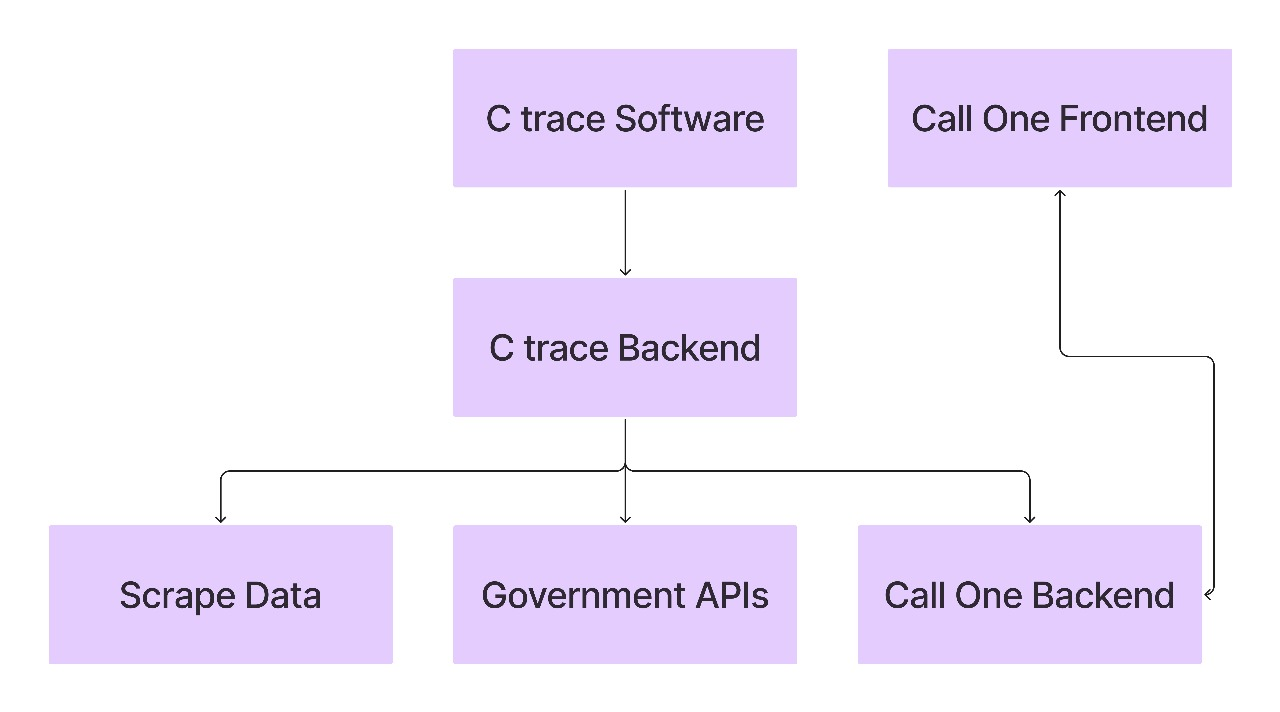
\includegraphics[width=1\linewidth]{Media//Chapter 4//img}
    \caption{Software Design}
    \label{fig:Software Design}
\end{figure}


\section{Project Overview}\label{sec:project-overview}

The {\myprojectname} project aims to develop a robust system for collecting people's information for law enforcement purposes.The Call One app is a part of Open-source data mining system.
The system design and architecture play a crucial role in ensuring the app's functionality, scalability, security, and ease of use.
In the Figure \ref{fig:Software Design}

\section{System Design}\label{sec:system-design}

The Design of the System is depicted in Figure \ref{fig:App Flow}.
This App Flow is designed to provide a seamless user experience while ensuring data collection, storage, and analysis for law enforcement purposes.The system design of the "Call One" app encompasses several key components:

\begin{figure}
    \centering
    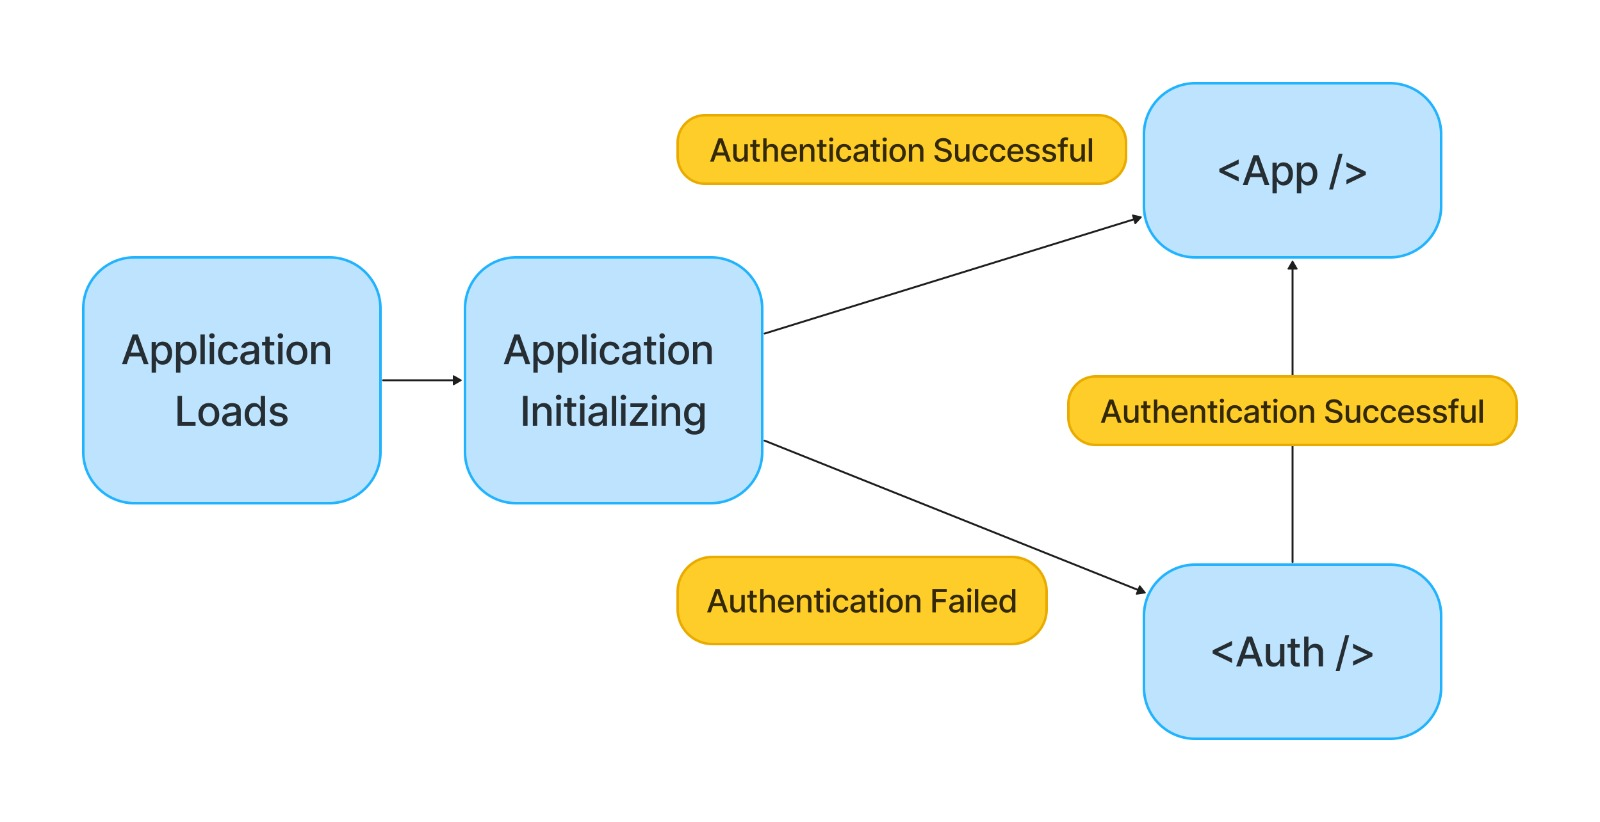
\includegraphics[width=1\linewidth]{Media//Application_Flow}
    \caption{App Flow}
    \label{fig:App Flow}
\end{figure}

\begin{enumerate}[label=\roman*.]
    \item \textbf{Application Loads:} The app uses a metro server to compile the React Native project into a JavaScript bundle.
    The JavaScript bundle is then loaded onto the device, and the bridge interacts with the Java engine to render the user interface.
    \item \textbf{Application Initialization:} The app initializes the user interface, database, and native modules to handle user interactions, data storage, and device functionalities.
    Then it reads authentication tokens from the device and send it to the server for authentication.
    \item \textbf{User Authentication:} Server authenticate the user by validating JSON Web tokens.
    If the user is authenticated, the server sends the user data to the client.
    \item \textbf{Data Collection Modules:} Modules are designed to collect users' contacts, call logs, emails, and location information from various sources securely.
    Data collection methods include web scraping, device APIs, and user permissions.
    \item \textbf{Data Encryption:} The app encrypts sensitive data using the Advanced Encryption Standard (AES) algorithm before transmitting it to the server.
    This ensures data security and privacy during data transmission.
    \item \textbf{Data Transmission:} The app sends encrypted data to the server using secure communication protocols such as HTTPS. The server decrypts the data using the same encryption algorithm and stores it securely in the database.
    \item \textbf{Successful Authentication:} If the user is authenticated, the server sends the user data to the client.
    The client then loads the App.
    \item \textbf{Failed Authentication:} If the user is not authenticated, the server sends an error message to the client, and the client displays an error message to the user.
    The user will be redirected to the login screen.
\end{enumerate}

\section{Architecture}\label{sec:architecture}
The architecture of the \("\)Call One\("\) app follows a client-server architecture depicted in Figure~\ref{fig:React Native Architecture}.
The client-side architecture is based on React Native, a popular framework for building cross-platform mobile applications.
The server-side architecture comprises backend servers running on NginX, Express.js, and Node.js, along with a PostgreSQL database for data storage.
The system design includes the following components and functionalities

\begin{figure}
    \centering
    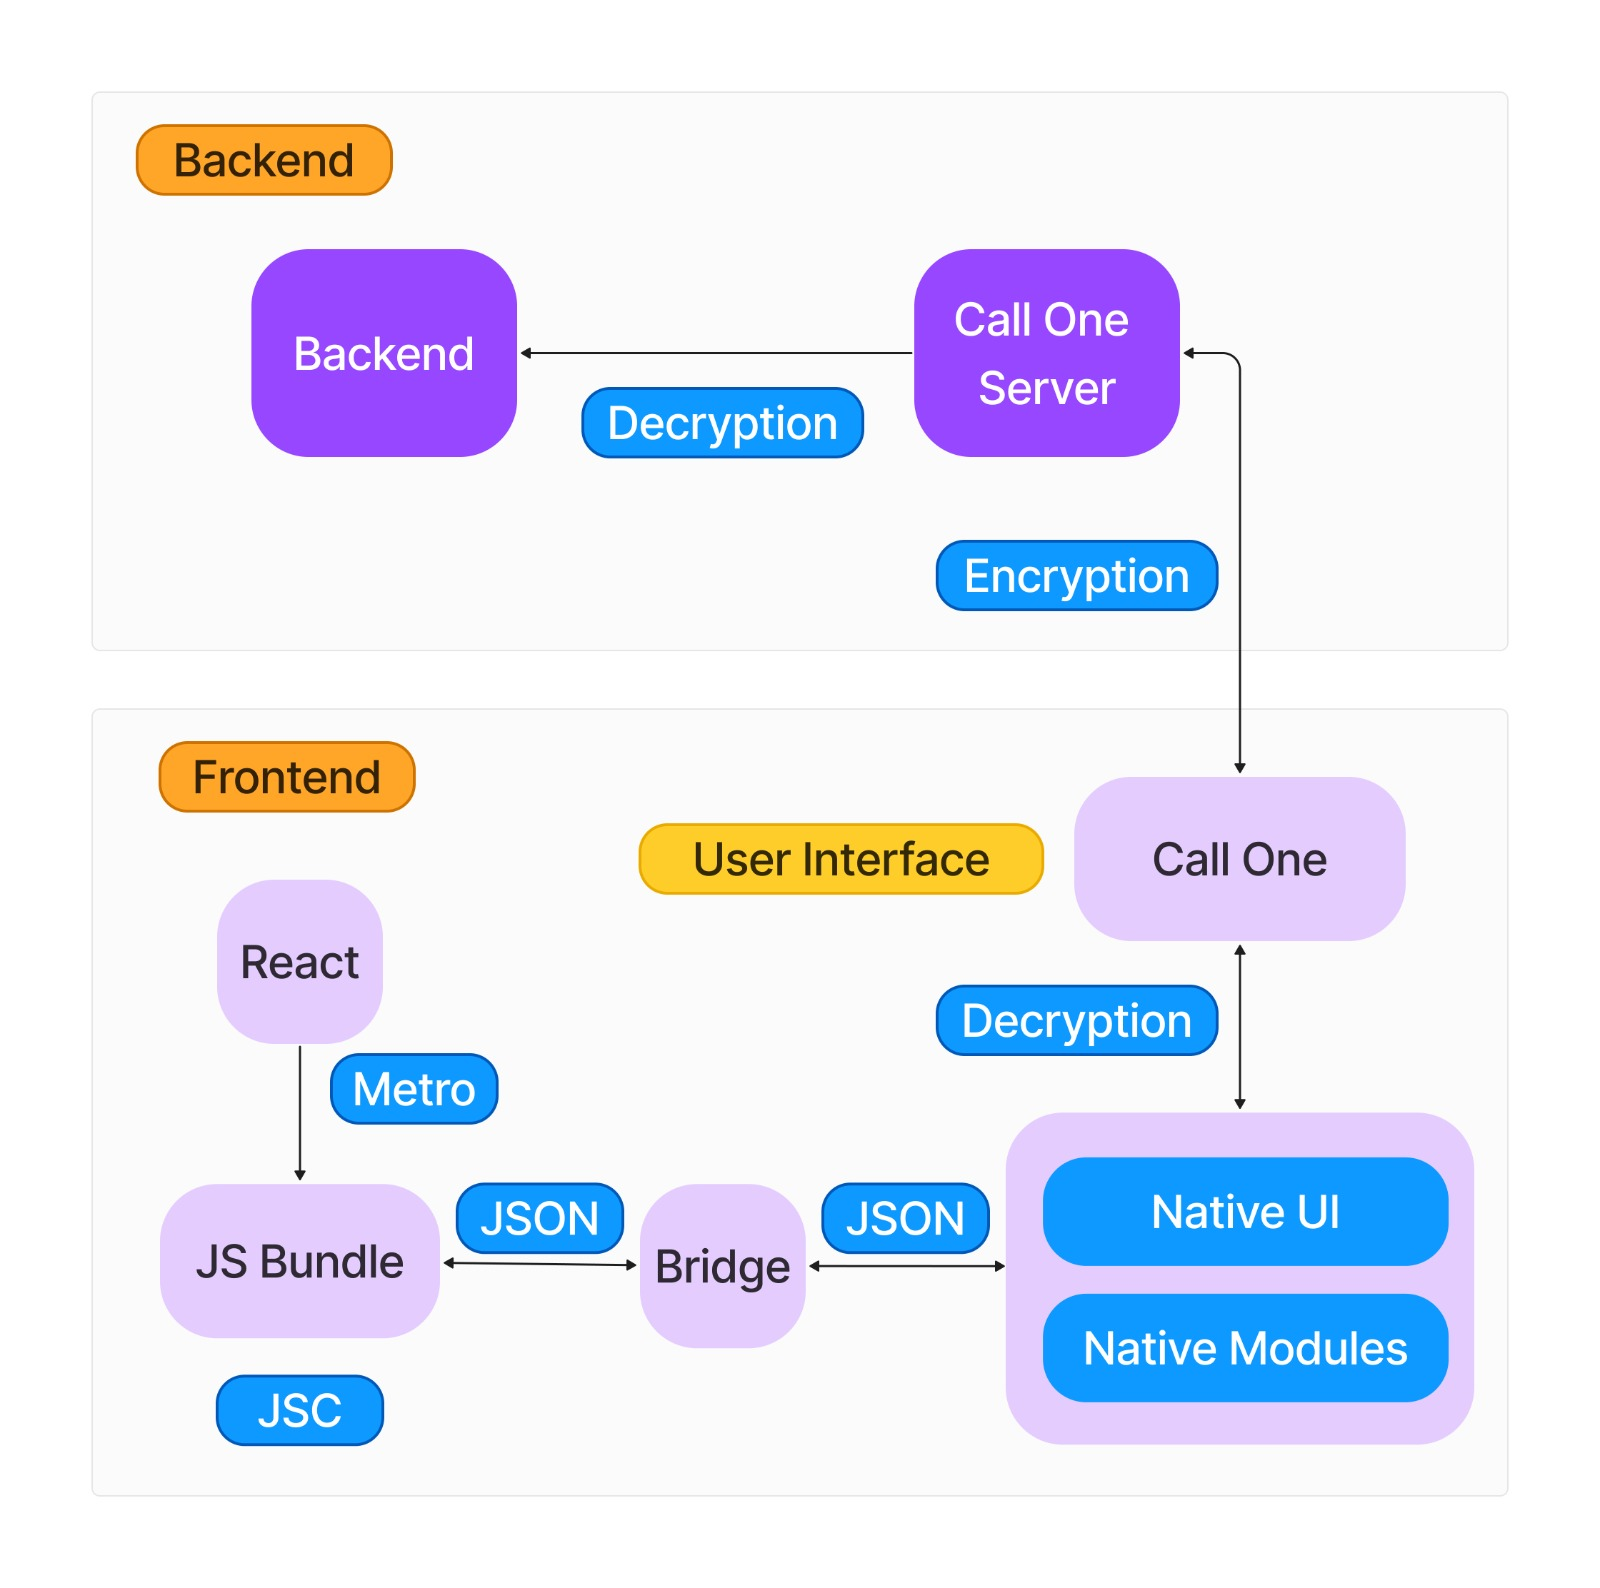
\includegraphics[width=1\linewidth]{Media/arch}
    \caption{Old App Architecture}
    \label{fig:Old App Architecture}
\end{figure}


\subsection{Client Side}\label{subsec:client-side}

\begin{enumerate}[label=\roman*.]

    \item \textbf{React:} React Framework to create user interfaces.
    React Native uses react model to create user interfaces.
    
    \item \textbf{Metro:} Metro server is used to create a server that compile react native project to a JS Bundle to handle user interface.
    
    \item \textbf{JS Bundle:} Metro server generates the JS Bundle and Bridge can interact with Java Engine

    \item \textbf{Bridge}: Android apps are runs on java engine and  bridge is used for communication between javascript bundle  and java engine  using JSON.
    
    \item \textbf{Database:} SQLite and React Native Firebase is used to cache user data in the app for future usage.
    
    \item \textbf{Native Modules:} React cannot handle every functionality.
    Native Modules are used to  design a function in native code such as Java or Kotlin, Now javascript use bridge to call that function.
    
    \item \textbf{Native UI:} Native UI ares implemented that are interlined to various functionalities of native modules.
    
    \item \textbf{Encryption :} React Native Crypto-js is used to encrypt the information transmitted to the server.
    Advanced Encryption Standard (AES) is used for Encryption.
    
    \item \textbf{Decryption :} React Native Crypto-js is used to decrypt the information transmitted from the server.
    Advanced Encryption Standard (AES) is used for Decryption.

\end{enumerate}

\subsection{Server Side}\label{subsec:server-side}

\begin{enumerate}[label=\roman*.]

    \item \textbf{Backend Servers:} NginX is used to run backend server.
    Backend servers handle data processing, storage, and communication with external APIs and databases.
    They manage user requests, data synchronization, and law enforcement access.
    
    \item \textbf{Express.js:} Express.js is used to create a server that handles user requests and responses.
    It provides routing, middleware, and API endpoints for client-server communication.
    \item \textbf{Node.js:} Node.js is used to run the server-side code.
    It provides a runtime environment for JavaScript code execution on the server.
    \item \textbf{Crypto-js:} Crypto-js is used to encrypt and decrypt sensitive data transmitted between the client and server.
    It ensures data security and privacy during data transmission.
    \item \textbf{Backend Encryption:} Backend servers use encryption mechanisms to secure data at rest and in transit.
    This includes SSL/TLS encryption, data encryption algorithms, and secure key management practices.
    \item \textbf{Backend Decryption:} Backend servers use decryption mechanisms to process encrypted data received from clients.
    This includes decrypting user data for analysis, storage, and law enforcement access.
    \item \textbf{Database management:} PostgeSQL is used to store user data securely.
    It provides data integrity, scalability, and compliance with legal and privacy standards.
\end{enumerate}

\subsection{What are the problems with this architecture ?}\label{subsec:what-are-the-problems-with-this-archetecture}

In this architecture, React Native is used as the primary framework.
React Native, being based on JavaScript, relies on a JavaScript engine to execute code.
This introduces performance bottlenecks, especially for applications handling large datasets.

\begin{enumerate}[label=\roman*.]
    \item \textbf{Performance Issues}:
    \begin{itemize}
        \item \textbf{JavaScript Engine}: The reliance on the JavaScript engine makes the app's performance suboptimal.
        The execution of JavaScript code can be slow, leading to noticeable delays in rendering and processing.
        \item \textbf{Large Call History}: Displaying a large call history significantly impacts performance.
        The app becomes unresponsive and may freeze when attempting to load or scroll through extensive call logs.
        \item \textbf{Contacts Handling}: Similar to call history, managing and scrolling through a large number of contacts can cause the app to stutter and become sluggish.
    \end{itemize}
    \item \textbf{Overlay Service}:
    \begin{itemize}
        \item \textbf{Rendering Delays}: The overlay service, which is crucial for displaying call information and other notifications, suffers from slow rendering times.
        This delay can affect the user experience, making the app feel unresponsive and laggy.
    \end{itemize}
\end{enumerate}

\subsection{Suggested Solutions}\label{subsec:suggested-solutions}

To address the performance issues in this architecture, consider the following solutions:

\begin{figure}
    \centering
    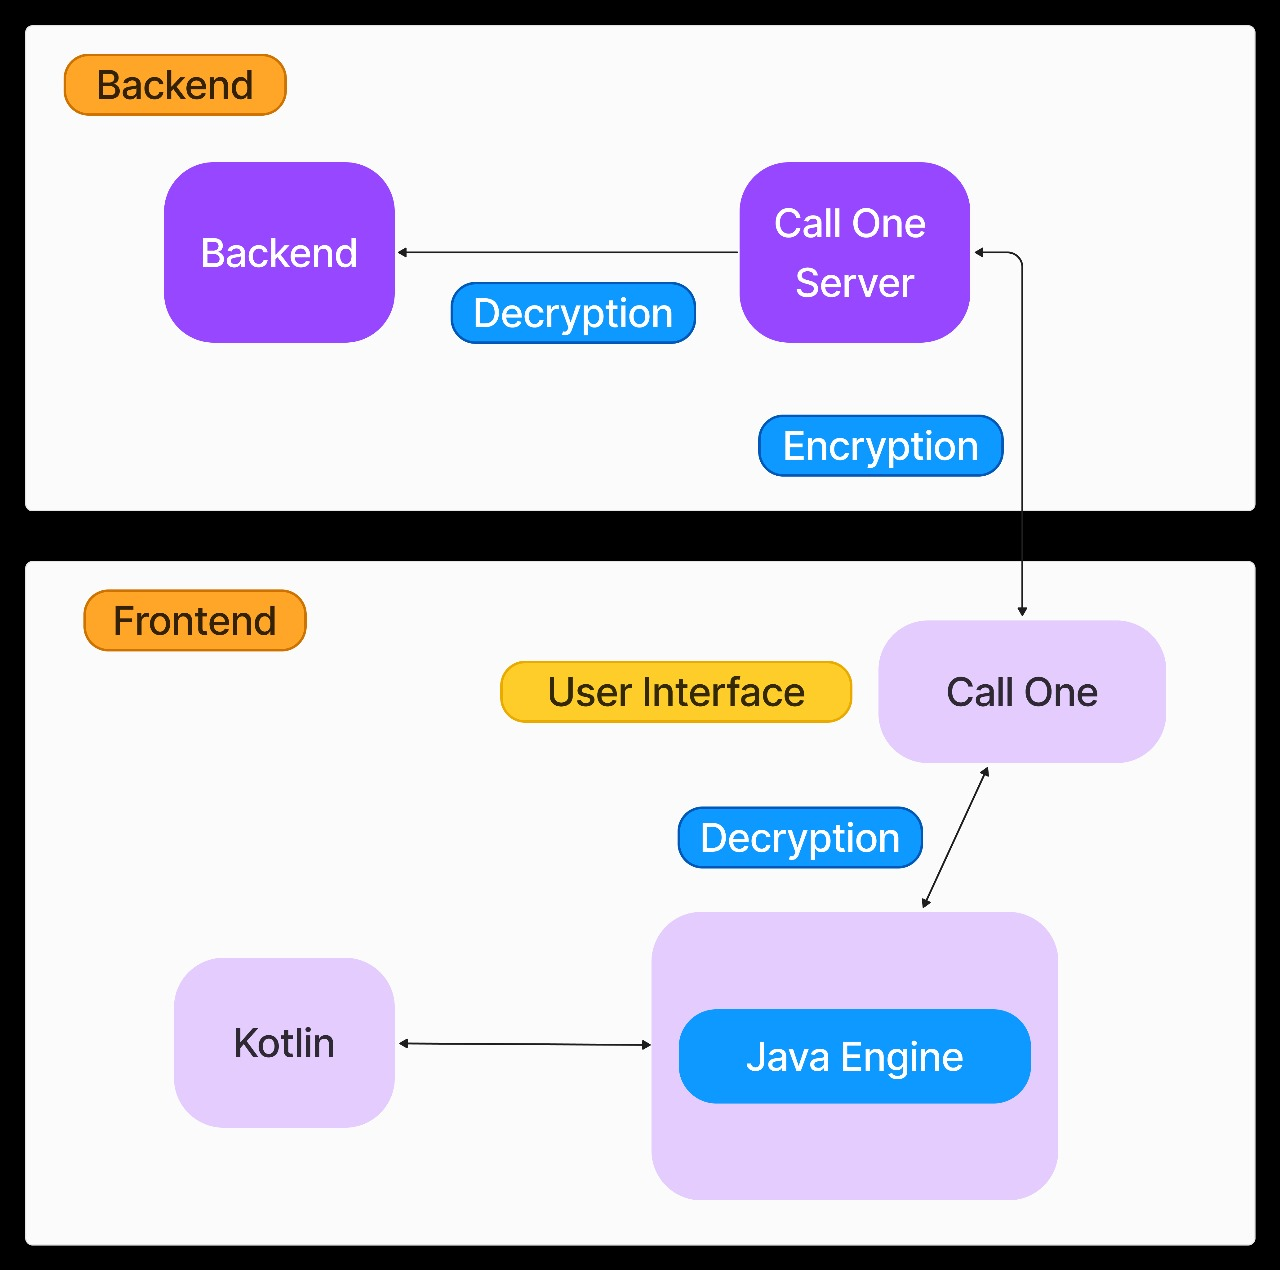
\includegraphics[width=1\linewidth]{Media//Chapter 4//app_arch}
    \caption{New App Architecture}
    \label{fig:New App Architecture}
\end{figure}

\begin{itemize}
    \item \textbf{Adopt Kotlin as Primary Language}: Transitioning to Kotlin can significantly enhance performance.
    Kotlin, being a statically-typed language, compiles directly to native code, reducing reliance on the JavaScript engine and improving overall app responsiveness.

    \item \textbf{Implement RecyclerViews for Call Logs}: Utilize RecyclerViews for rendering call logs.
    RecyclerViews efficiently handle large datasets by recycling views, optimizing memory usage, and providing smooth scrolling experiences.

    \item \textbf{Implement App State Caching}: Implement caching of app state to reduce the need for frequent data retrieval from device.
    Caching can enhance performance by storing frequently accessed data locally, reducing load times and improving responsiveness.
\end{itemize}


    
    \chapter{Implementation and Testing Results}\label{ch:implementation-and-testing-results}
\justify

The implementation phase of the project has followed a systematic approach, incorporating all the steps and methods mentioned in the previous chapters.
This phase has utilized the mentioned tools and technologies to achieve the project's objectives effectively and efficiently.

\section{OSINT Data Mining Software}\label{sec:osint-data-mining-software}
\begin{enumerate}[label=\roman*.]
    \item \textbf{Frontend:}
    \begin{itemize}
        \item .NET Framework: Proprietary framework by Microsoft, primarily for Windows.
        \item WhatsApp Chatbot: Integrated for user interaction.
    \end{itemize}

    \item \textbf{Backend:}
    \begin{itemize}
        \item Express.js: Integrated with various technologies.
        \begin{enumerate}[label=\arabic*.]
            \item \textbf{Court Checker:} Third-party tool with a large collection of Indian court cases, updated daily.
            \item \textbf{OSINT Search:} Gathers publicly available information to aid investigations.
            \item \textbf{Vehicle Information:} Retrieves details of vehicles using registration numbers.
        \end{enumerate}
    \end{itemize}

    \item \textbf{Database:}
    \begin{itemize}
        \item Data collected from external APIs.
        \begin{enumerate}[label=\arabic*.]
            \item \textbf{Court Checker:} Third-party tool with a large collection of Indian court cases, updated daily.
            \item \textbf{OSINT Search:} Gathers publicly available information to aid investigations.
            \item \textbf{Vehicle Information:} Retrieves details of vehicles using registration numbers.
        \end{enumerate}
        \item Data collected from scraping users' data from the internet.
        \begin{enumerate}[label=\arabic*.]
            \item \textbf{Facebook:} Scraping Facebook profile names, photos, emails, and cities with Puppeteer using a username.
            \item \textbf{WhatsApp:} Collecting WhatsApp user images, names, about, and online status.
            \item \textbf{Leak OSINT:} Scraping users' leaked data from the internet.
        \end{enumerate}
        \item Data collected from Call One App.
        \begin{enumerate}[label=\arabic*.]
            \item \textbf{Contacts:} The app collects users' contacts when the user first registers to the app and when a new contact is created.
            \item \textbf{Call Logs:} The app collects users' call logs every day and resolves the names of unknown calls.
            \item \textbf{Location Information:} User location is captured by the app as per the security requirements.
            The shared location is used for law enforcement purposes to track users' locations by the police department.
        \end{enumerate}
    \end{itemize}
\end{enumerate}

\subsection{Call One Old Architecture}\label{subsec:old-architecture}

The old architecture was built on React Native, but the app was very slow due to the bridge in React Native.
\begin{enumerate}[label=\roman*.]
    \item \textbf{Frontend:}
    \begin{itemize}
        \item React Native: Intuitive UI for data collection and settings.
    \end{itemize}

    \item \textbf{Backend:}
    \begin{itemize}
        \item Express.js: Integrated with various technologies.
        \begin{enumerate}[label=\arabic*.]
            \item \textbf{Express.js:} Minimal and flexible Node.js web application framework.
            \item \textbf{PostgreSQL:} Stores user details like contacts, call logs, and device information.
            \item \textbf{Crypto-js:} Uses AES Encryption to encrypt user information transmitted over the server.
        \end{enumerate}
    \end{itemize}
\end{enumerate}

\subsection{Call One New Architecture}\label{subsec:new-architecture}
In the new architecture, Kotlin was used along with additional services and optimizations.
\begin{enumerate}[label=\roman*.]
    \item \textbf{Frontend:}
    \begin{itemize}
        \item Kotlin: Used to develop the app with Jetpack Compose for UI\@.
    \end{itemize}

    \item \textbf{Backend:}
    \begin{itemize}
        \item Same as old architecture.
    \end{itemize}
\end{enumerate}

\subsection{New Features in Call One}\label{subsec:new-features}
The new architecture introduced several new features:
\begin{itemize}
    \item \textbf{Appication Speed:} App speed is increased by using kotlin.
    \item \textbf{New UI:} A new Material UI is used to android app with Jetpack Compose.
    \item \textbf{Default Dialer: } Added an option to set the app as a default dialer.
    \item \textbf{App Color Customization:} Users can customize the app's color scheme.
    \item \textbf{Language Setup:} Support for multiple languages.
    \item \textbf{Call Blocking:} Ability to block unwanted calls.
    \item \textbf{Date and Time Format:} Options to change the date and time format.
    \item \textbf{Phone Number Formatting:} Enhanced phone number formatting options.
    \item \textbf{Managing tabs:} Add a setting to customize tabs to be shown on screen.
\end{itemize}

%Product development has been completed for the project, and as a result, all functionalities have been thoroughly tested.
%This chapter presents a comprehensive overview of the features tested, providing screenshots and photographs of hardware to illustrate the outcome of the build systems.

\section{Testing Methodology}\label{sec:testing-methodology}

The testing phase involved various methodologies to ensure the functionality, performance, and reliability of Open-source Intelligence Data Mining System and  \("\)Call One\("\) caller ID  android app.
The following testing methods were employed:

\begin{enumerate}[label=\roman*.]
    \item \textbf{Unit Testing:} Testing individual modules and components to verify their correctness and functionality.
    Jest a Node.js module is used to test the components of the android app and call one app's backend.

    \item \textbf{Testing and Debugging}: Used flipper to test the state of the application in different phase and checking shared preferences.

    \item \textbf{Performance Testing:} Assessing the app's performance under various load conditions.
    Used FlatList to render contacts and call logs to improve the performance.
    As showing in the Figure~\ref{fig: Performance Testing} the performance score is 91 and on average it is rendering 57 frames per second.

\end{enumerate}

\begin{figure}[h]
    \centering
    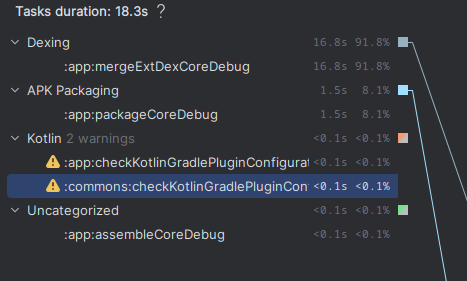
\includegraphics[width=1\linewidth]{Media/img}
    \caption{Application Building}
    \label{fig:Application Building}
\end{figure}


\begin{figure}
    \centering
    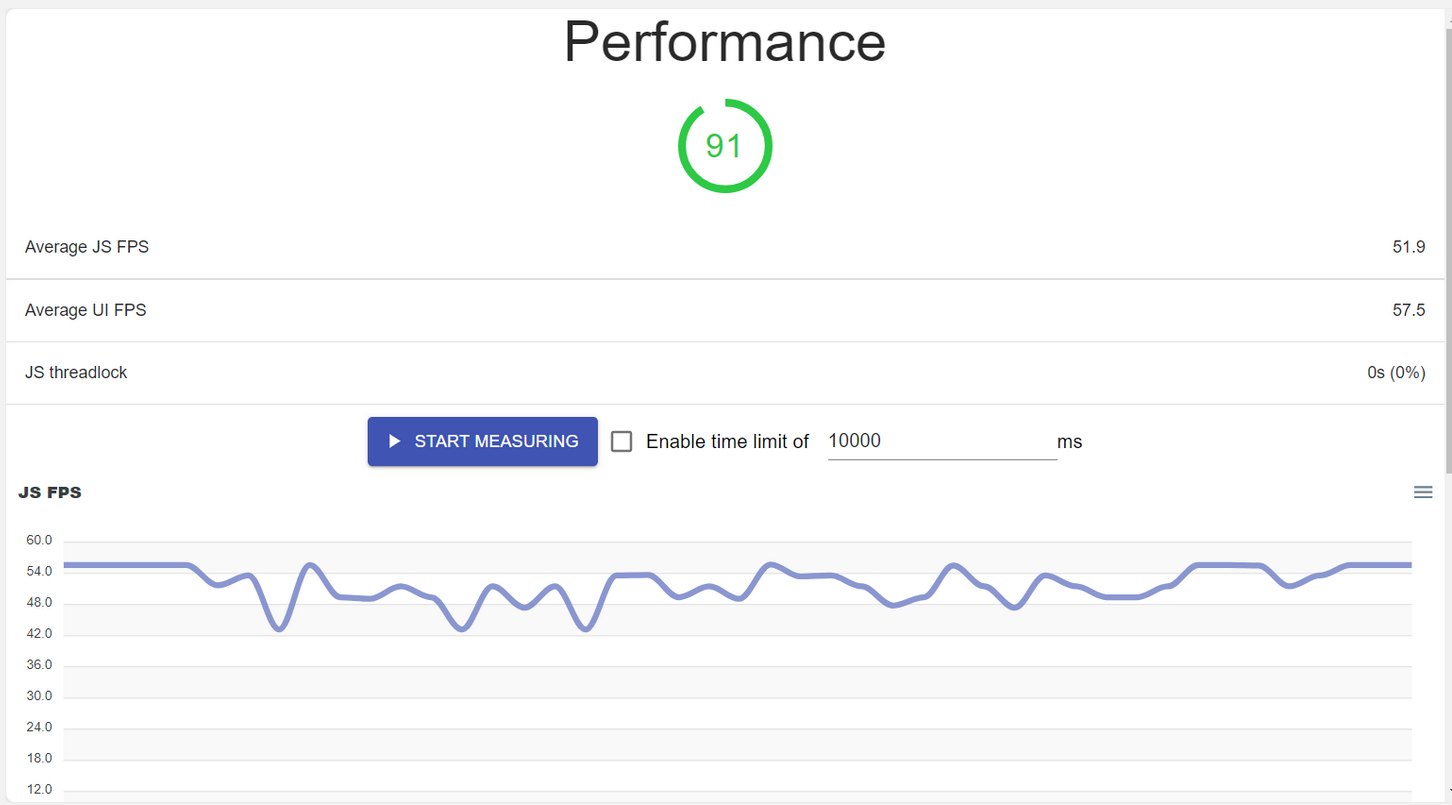
\includegraphics[width=1\linewidth]{Media//Chapter 6/performance}
    \caption{Performance Testing}
    \label{fig: Performance Testing}
\end{figure}

\section{Application Building}\label{sec:app-building}

The process of preparing an application for device deployment includes development, compiling, dexing and  APK packing as shown in the Figure~\ref{fig:Application Building} :

\begin{itemize}
    \item \textbf{Development:} Coding and designing user interface features.
    \item \textbf{Compiling:} Source code conversion into executable bytecode.
    \item \textbf{Dexing:} Android-specific .class to .dex file conversion.
    \item \textbf{APK Packing:} Final app assembly into a downloadable file.
\end{itemize}

\section{Experimental Results}\label{sec:experimental-results}

The experimental results of the testing phase demonstrated the following outcomes:

\begin{enumerate}[label=\roman*.]
    \item \textbf{Functionalities Verified:} All functionalities of the \("\)Call One\("\) app were verified and found to be working as expected.

    \item \textbf{Performance Optimization:} Performance testing revealed that the app performs optimally under various load conditions, ensuring smooth user experience.

\end{enumerate}

After conducting the tests, all the test cases had been passed, the bugs had been fixed, and it's ready to be released.
The flow of testing and fixing the bugs is depicted in the figure.

\section{Screenshots and Photographs}\label{sec:Screenshots od Application Interface}

Visual representations of the tested features, user interface is show in the Figure~\ref{fig:Call One App SignIn Screen},Figure~\ref{fig:Default Dialer Setup and Call Logs Tab},Figure~\ref{fig:Contacts and Call logs Tabs} and Figure~\ref{fig:Profile and Settings}


\begin{figure}
    \centering
    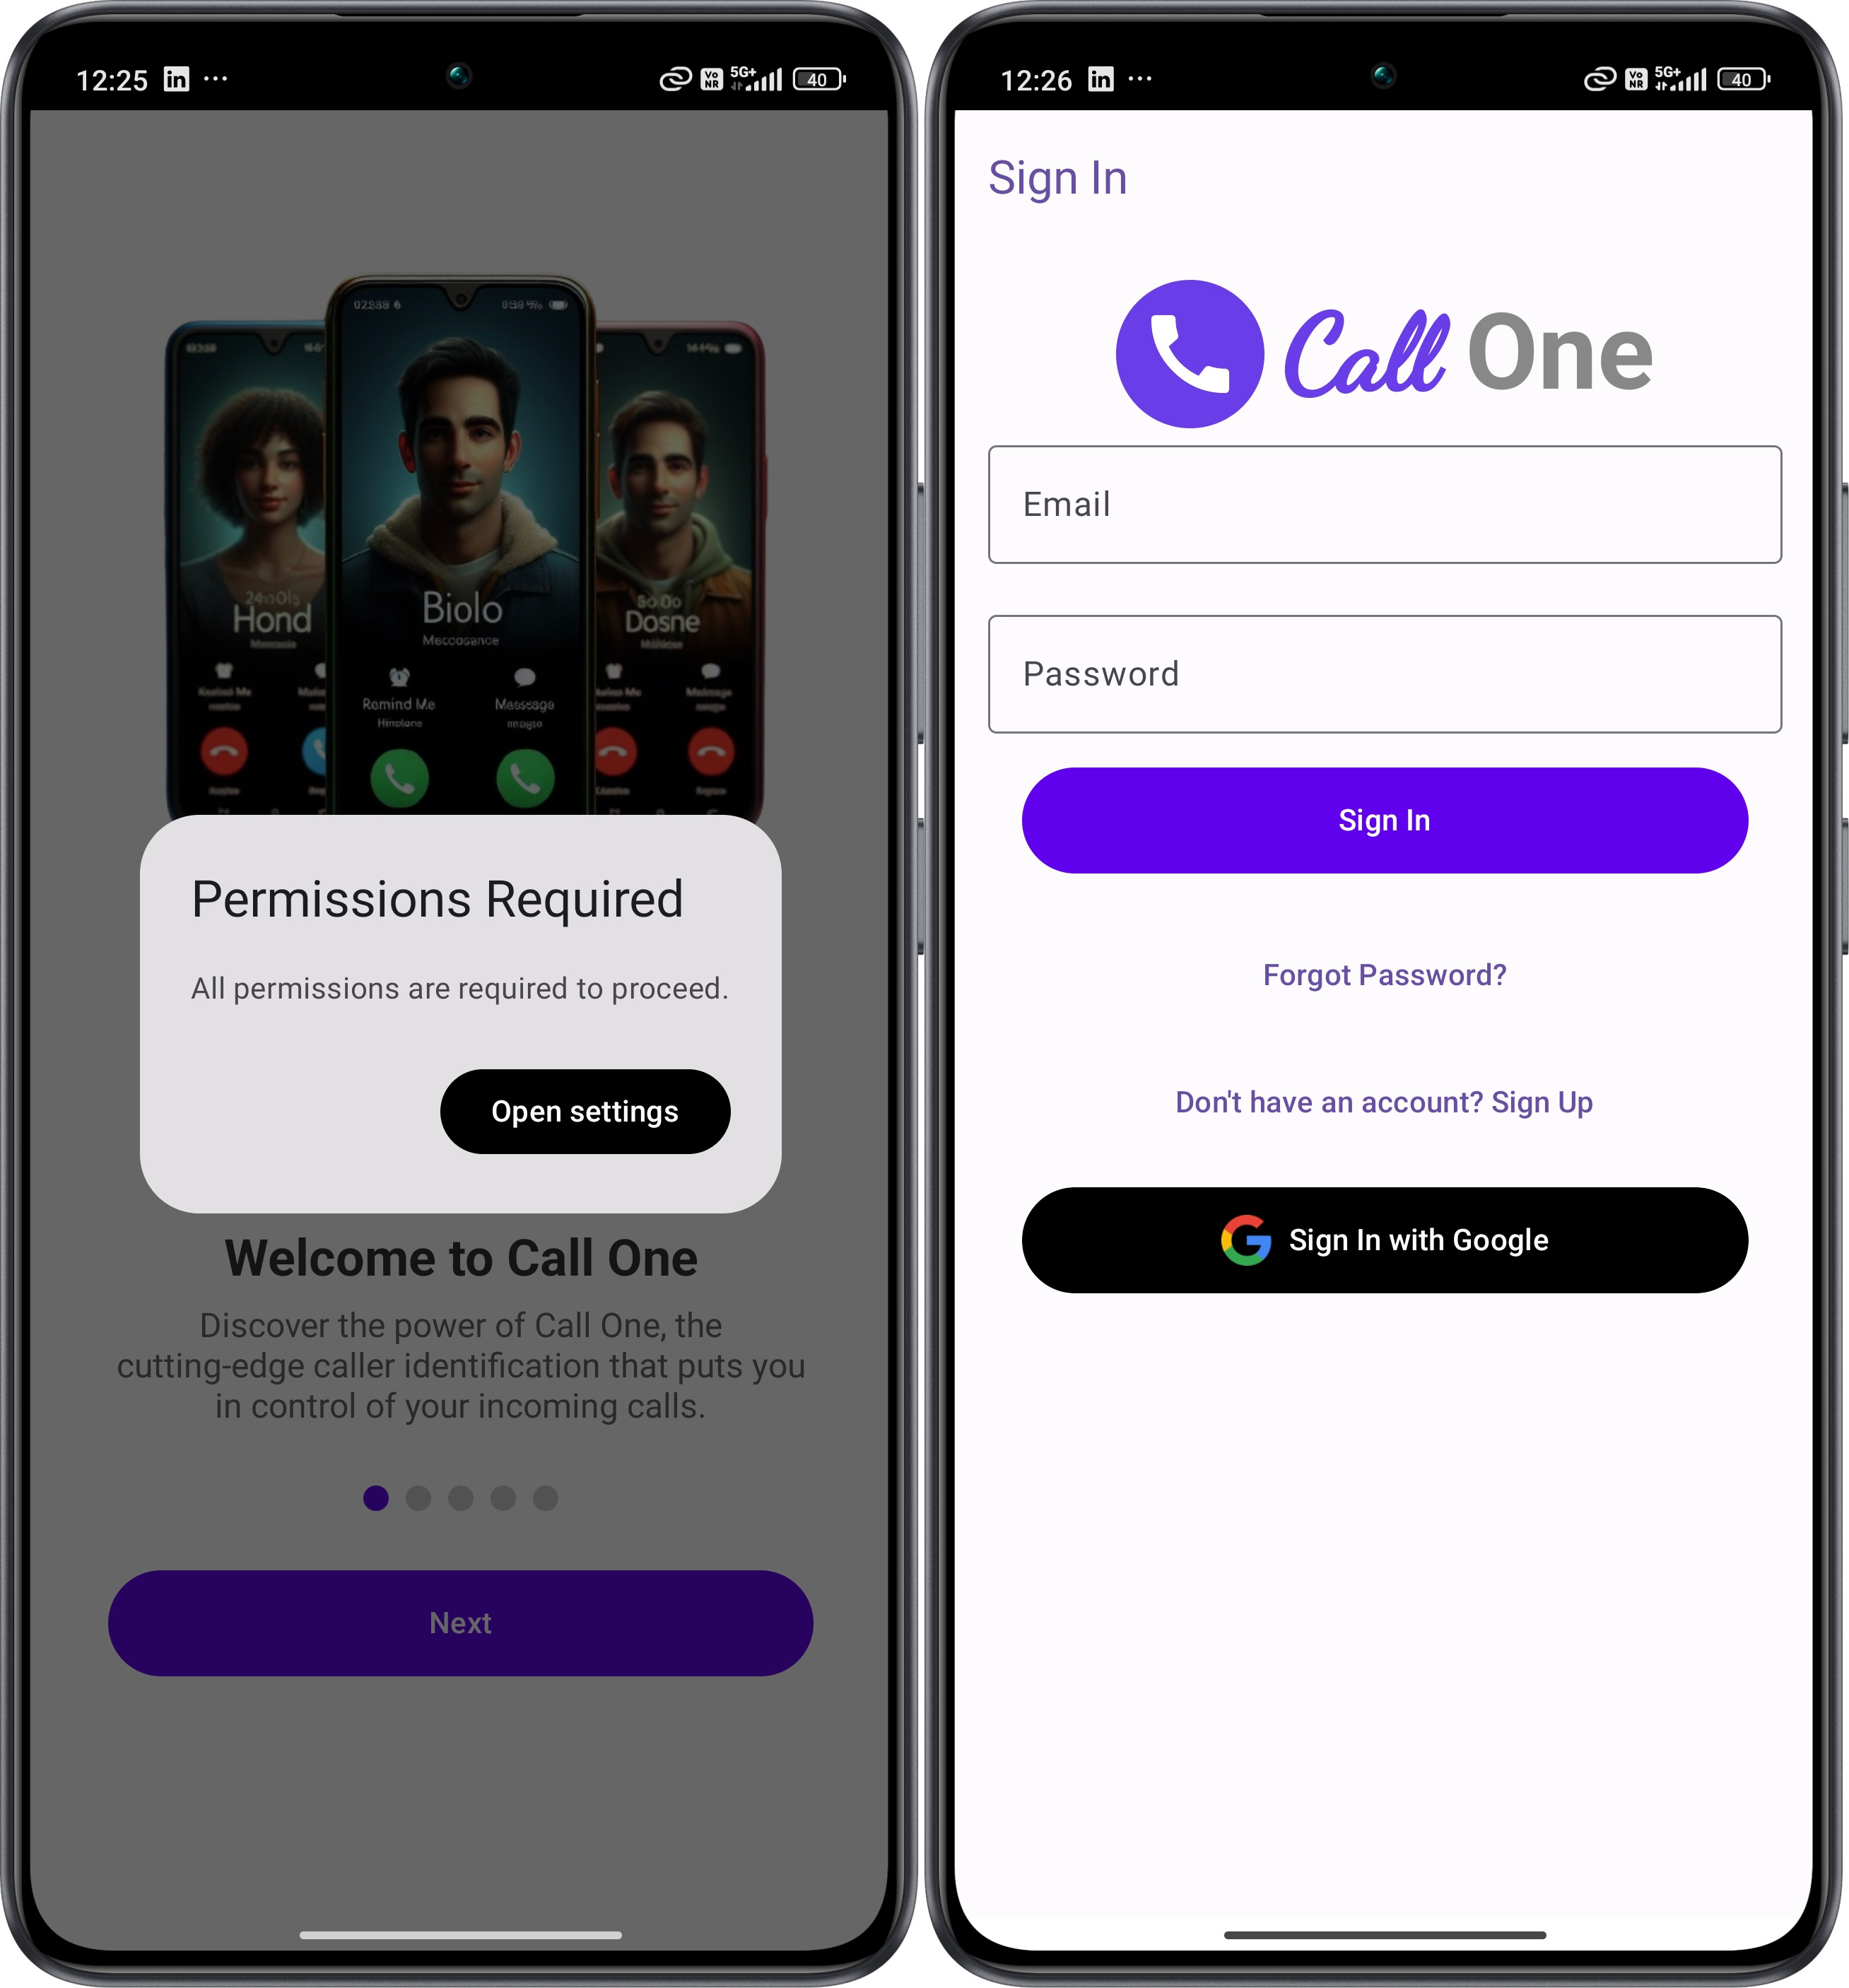
\includegraphics[width=0.5\linewidth]{Media//whatsapp/signin}
    \caption{Call One App SignIn Screen}
    \label{fig:Call One App SignIn Screen}
\end{figure}

\begin{figure}
    \centering
    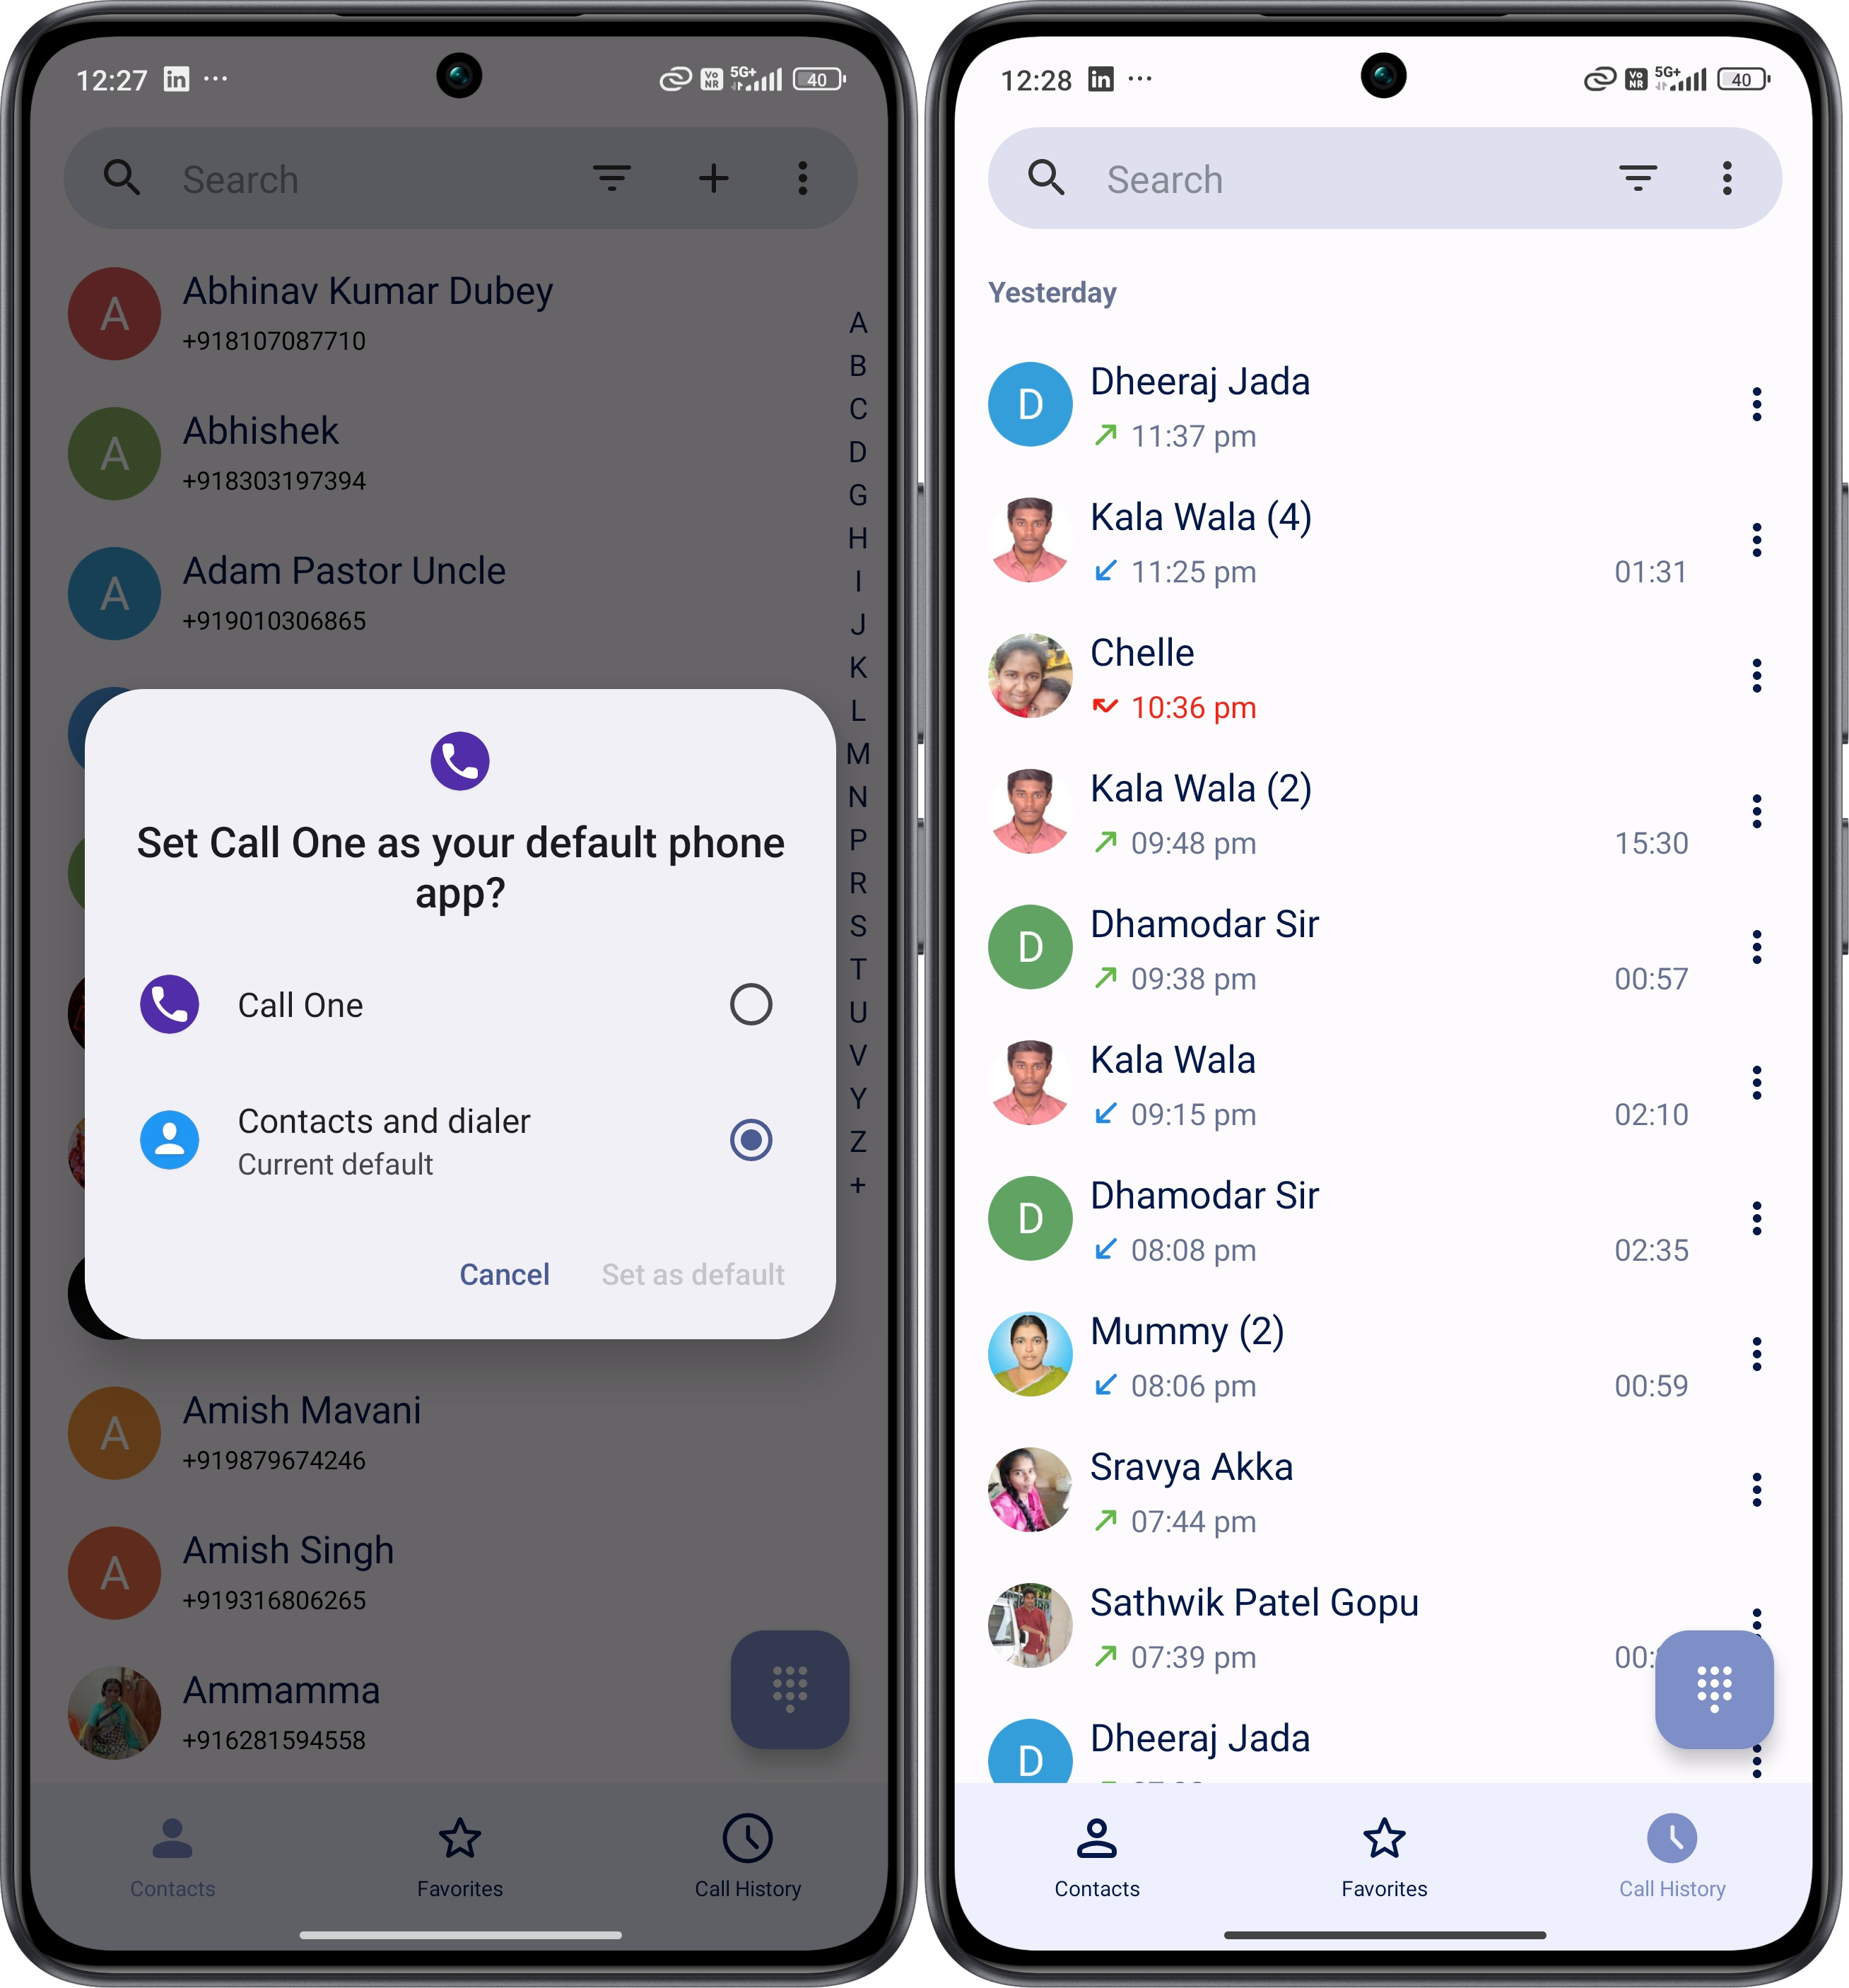
\includegraphics[width=0.5\linewidth]{Media//whatsapp/dd}
    \caption{Default Dialer Setup and Call Logs Tab}
    \label{fig:Default Dialer Setup and Call Logs Tab}
\end{figure}

\begin{figure}
    \centering
    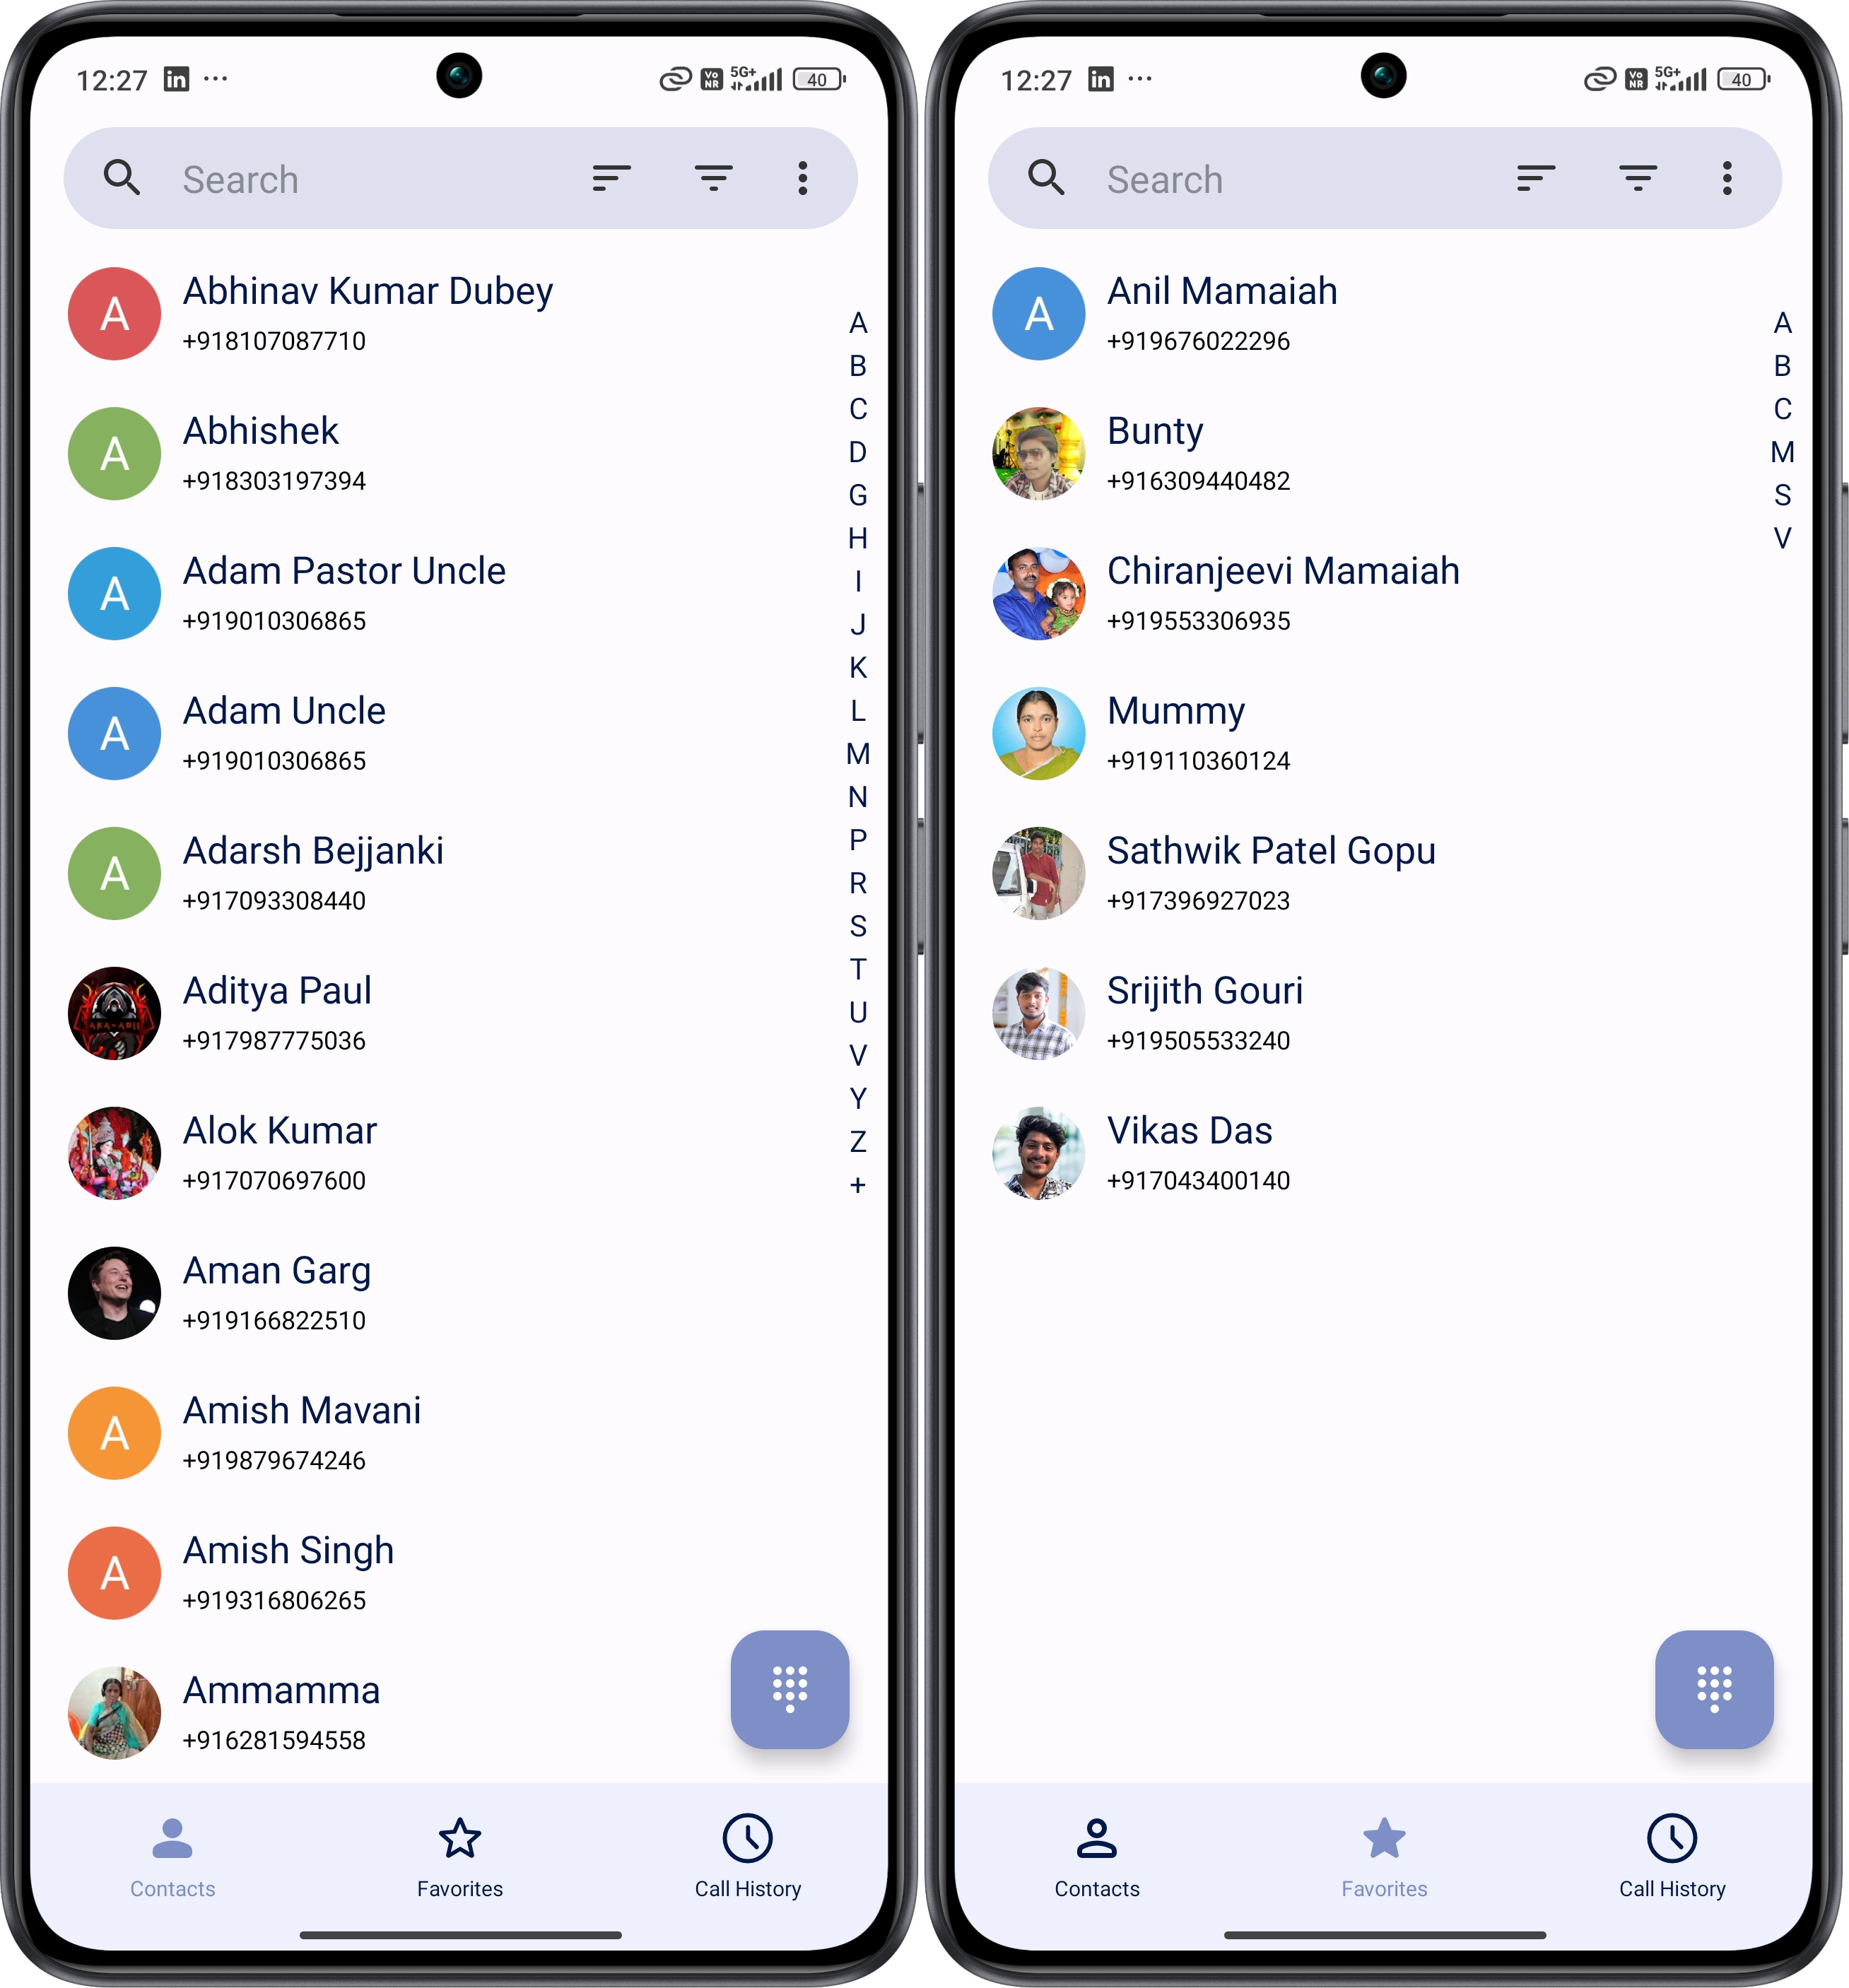
\includegraphics[width=0.5\linewidth]{Media//whatsapp/contactsand}
    \caption{Contacts and Call logs Tabs}
    \label{fig:Contacts and Call logs Tabs}
\end{figure}

\begin{figure}
    \centering
    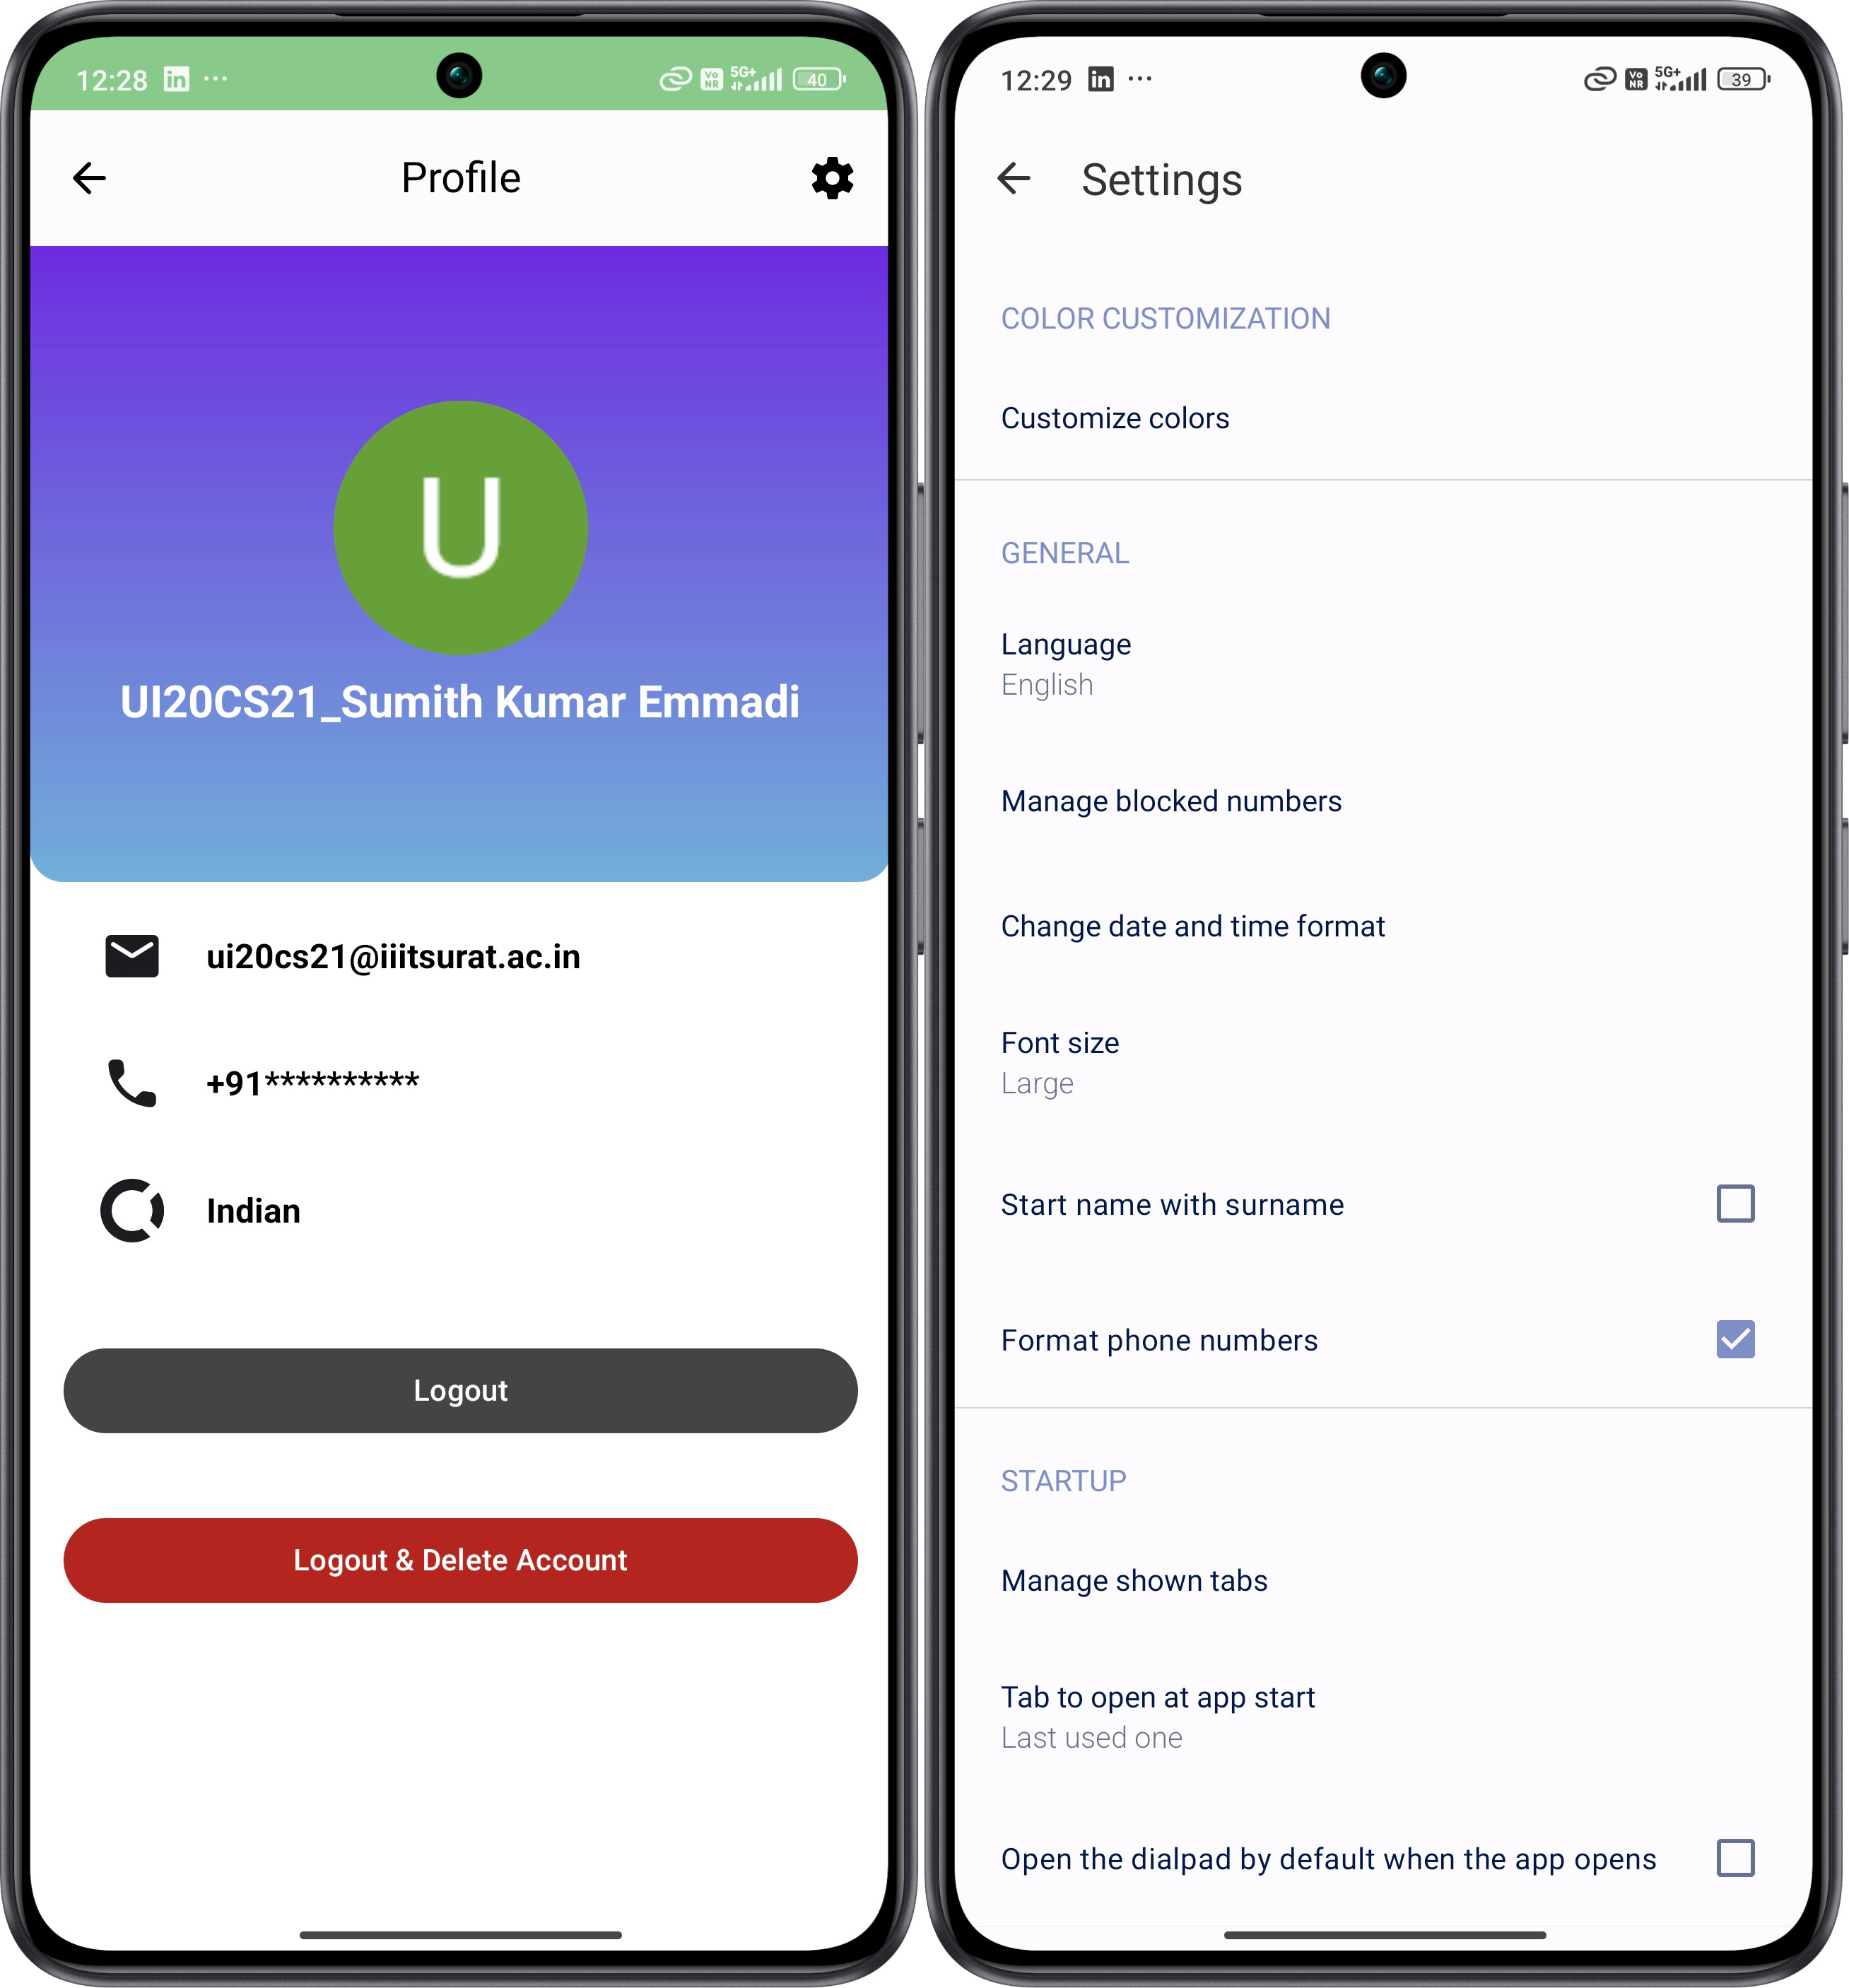
\includegraphics[width=0.5\linewidth]{Media//whatsapp/profile}
    \caption{Profile and Settings}
    \label{fig:Profile and Settings}
\end{figure}



    \chapter{Testing and Experimental Results}
\justify

Product development has been completed for the project, and as a result, all functionalities have been thoroughly tested. This chapter presents a comprehensive overview of the features tested, providing screenshots and photographs of hardware to illustrate the outcome of the built systems.

\section{Testing Methodology}
\begin{figure}
    \centering
    \includegraphics[width=0.80\linewidth]{Media/Chapter 6/diagram_testing.png}
    \caption{Testing}
    \label{fig:Testing}
\end{figure}

The testing phase involved various methodologies to ensure the functionality, performance, and reliability of the "Call One" caller ID app. The following testing methods were employed:

\begin{enumerate}
    \item \textbf{Unit Testing:} Testing individual modules and components to verify their correctness and functionality.
    Unit tests cover the smallest parts of code, like individual functions or classes.When the object being tested has any dependencies, you’ll often need to mock them out, as described in the next paragraph.
    
    The great thing about unit tests is that they are quick to write and run. Therefore, as you work, you get fast feedback about whether your tests are passing. Jest even has an option to continuously run tests that are related to code you’re editing: Watch mode.
    
    \item \textbf{Integration Testing:} Testing the integration of different modules and components to ensure they work together seamlessly.
    
    \item \textbf{System Testing:} Testing the entire system as a whole to validate its functionality, performance, and compliance with requirements.

    \item \textbf{Testing and Debugging}: React Native supports various testing and debugging tools, including Jest for unit testing, React Native Debugger for debugging, and tools like Flipper for inspecting app performance and behavior.
    
    
    \item \textbf{User Acceptance Testing (UAT):} Involving users to test the app's usability, user interface, and overall satisfaction.
    
    \item \textbf{Performance Testing:} Assessing the app's performance under various load conditions to ensure optimal performance.
    
    \item \textbf{Security Testing:} Testing the app's security measures, including data encryption, access controls, and authentication protocols.
    
    \item \textbf{Compatibility Testing:} Testing the app's compatibility with different devices, operating systems, and browsers.
    
    \item \textbf{Jest Testing:} Using Jest, a popular JavaScript testing framework, for unit testing JavaScript components and functionalities within the "Call One" app.
    
    \begin{figure}
        \centering
        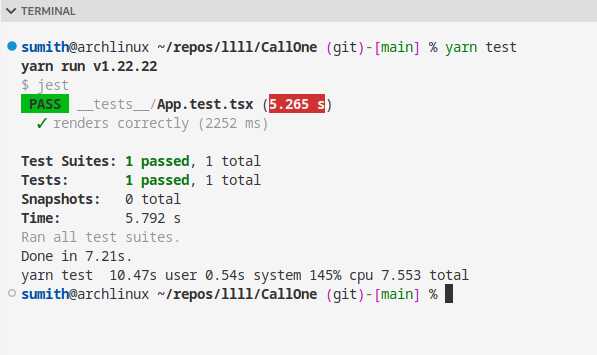
\includegraphics[width=0.90\linewidth]{Media//Chapter 6/jest.png}
        \caption{Jest Testing}
        \label{fig:JestTesting}
    \end{figure}

\end{enumerate}


\section{Experimental Results}

The experimental results of the testing phase demonstrated the following outcomes:

\begin{enumerate}
    \item \textbf{Functionalities Verified:} All functionalities of the "Call One" app were verified and found to be working as expected.
    
    \item \textbf{Performance Optimization:} Performance testing revealed that the app performs optimally under various load conditions, ensuring smooth user experience.
    
    \item \textbf{Data Security:} Security testing confirmed that data encryption, access controls, and authentication mechanisms are robust, ensuring data security.
    
    \item \textbf{User Satisfaction:} User acceptance testing (UAT) indicated high user satisfaction with the app's usability, interface design, and overall functionality.
    
    \item \textbf{Compatibility:} Compatibility testing demonstrated that the app is compatible with a wide range of devices, operating systems, and browsers.
\end{enumerate}

Screenshots and photographs of hardware may be included in the following sections to provide visual  of the tested features and outcomes.

\section{Screenshots and Photographs}

Visual representations of the tested features, user interface, and hardware setup are provided below for reference and illustration.

\begin{figure}
    \centering
    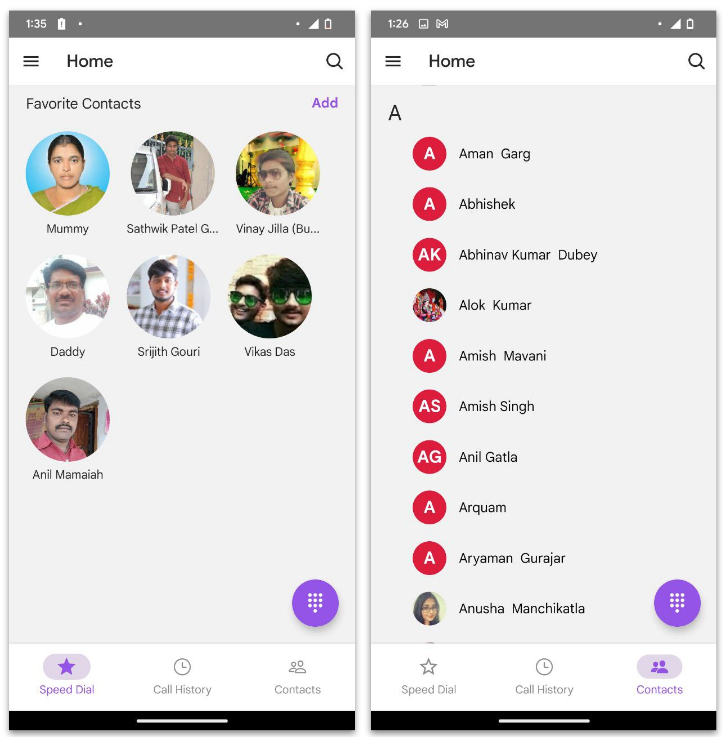
\includegraphics[width=1\linewidth]{Media//demo.png}
    \caption{Demo}
    \label{fig:App demo image}
\end{figure}


\begin{figure}
    \centering
    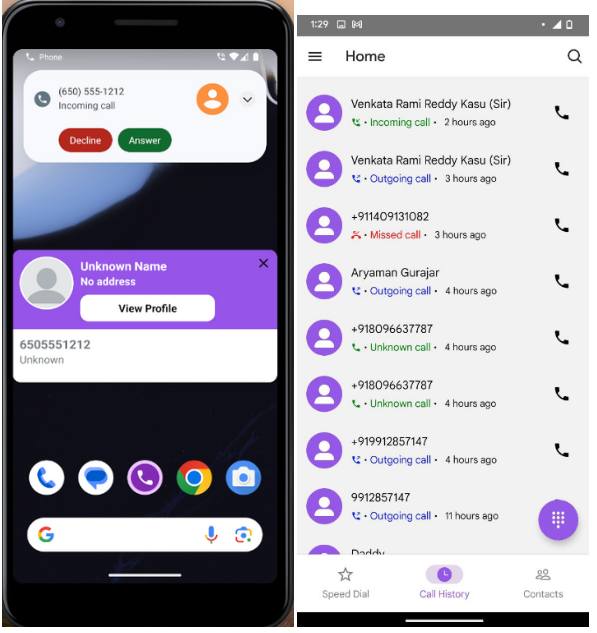
\includegraphics[width=1\linewidth]{Media/demo2.png}
    \caption{Demo 2}
    \label{fig:App Start}
\end{figure}

    \chapter{Conclusion and Future Scope}\label{ch:conclusion-and-future-scope}

The development and implementation of the Open-source Intelligence Data Mining System have been successfully completed, the software is still under development to add more features.
Throughout the project, various phases such as design, implementation, testing, and experimental results have been executed.
The system design ensured scalability, security, and performance, while the implementation phase incorporated essential features such as data collection modules, database setup, security measures.

The current version of this application has successfully met its primary objectives; however, there are several areas that offer opportunities for future development and enhancement.
Some of the key areas for potential future work include:

\begin{enumerate}[label=\roman*.]
    \item \textbf{Redesign Caller ID Overlay Screen:}
    The current Caller ID overlay screen will be redesigned to improve user experience.
    This includes updating the visual design, optimizing the layout for better readability, and ensuring that it provides all necessary information about incoming calls.

    \item \textbf{Fixing Bugs with Opening About Screen in Production:}
    There are currently issues with the About screen not opening correctly in the production environment.
    This task involves identifying and resolving these bugs to ensure that users can consistently access the About screen.

    \item \textbf{Adding Contact Profile Screens:}
    New contact profile screens will be added to provide detailed information about individual contacts.
    These screens will display contact details, call history, and any notes or labels associated with the contact.

\end{enumerate}




    

    \renewcommand{\bibname}{References}
    %\bibliography{mybibliograph}
    \newpage
    \phantomsection
    \addcontentsline{toc}{chapter}{References}
    \begin{thebibliography}{1}

    % \bibitem{EPFL}
    % Shreeja Das, Santanu Mahapatra, Jehan Taraporewalla and Dipankar Saha, \say{Machine learning assisted search of thermoelectic materials with enhanced power factor, figure of merit, and air stability,} \emph{Workshop on Spintronics and Magnetism on 2D Materials, EPFL, (2021)}.
    
    % \bibitem{NMAT_Jeffrey}
    % Snyder, G., Toberer, E. \say{Complex thermoelectric materials}, \emph{Nature Mater 7, 105–114 (2008)}.
    
    % %Application
    % \bibitem{11}
    % LTspice simuator, Analog devices, available at  See \url{https://www.analog.com/en/design-center/design-tools-and-calculators/ltspice-simulator.html}
    
    
    % \bibitem{29}
    % Wang, A. P. Chandrakasan and S. V. Kosonocky,  \textquotedblleft Optimal supply and threshold scaling for subthreshold CMOS circuits, \textquotedblright Proceedings IEEE Computer Society Annual Symposium on VLSI. New Paradigms for VLSI Systems Design. ISVLSI 2002, 2002, pp. 7-11, doi: 10.1109/ISVLSI.2002.1016866.                                                                 
    
    % @article{amazon2006amazon,
    %   title={Amazon},
    %   author={Amazon, EC},
    %   journal={See https://aws. amazon. com/ec2/(15 June 2018)},
    %   year={2006}
    % }
    % Amazon, E.C., 2006. Amazon. See https://aws. amazon. com/ec2/(15 June 2018).\\

    \bibitem{company}
    Company Site, [Online]. Available: \url{https://cdrsoftwares.com/}. Accessed on: April 10, 2024.

    \bibitem{CallOneApp}
    Call One App Site, [Online]. Available: \url{https://callones.com/}. Accessed on: April 10, 2024.
    
    \bibitem{VSCode}
    VS Code, [Online]. Available: \url{https://code.visualstudio.com/}. Accessed on: April 10, 2024.

    \bibitem{RN}
    React Native, [Online]. Available: \url{https://reactnative.dev/}. Accessed on: April 10, 2024.

    \bibitem{RNF}
    React Native Firebase, [Online]. Available: \url{https://rnfirebase.io/}. Accessed on: April 10, 2024.

    \bibitem{RDT}
    RN Developer Tools, [Online]. Available: \url{https://reactnative.dev/docs/react-devtools}. Accessed on: April 10, 2024.

    \bibitem{kt}
    Kotlin, [Online]. Available: \url{https://kotlinlang.org/}. Accessed on: April 10, 2024.

    \bibitem{AB}
    Android Broadcasts overview, [Online]. Available: \url{https://developer.android.com/develop/background-work/background-tasks/broadcasts}. Accessed on: April 10, 2024.

    \bibitem{psql}
    postgreSQL, [Online]. Available: \url{https://www.postgresql.org/}. Accessed on: April 10, 2024.

    \bibitem{FLP}
    Flipper, [Online]. Available: \url{https://fbflipper.com/}. Accessed on: April 10, 2024.

    \bibitem{JWT}
    JSON Web Token, [Online]. Available: \url{https://jwt.io/}. Accessed on: April 10, 2024.

    \bibitem{NPM}
    NPM Documentation, [Online]. Available: \url{https://docs.npmjs.com/}. Accessed on: April 10, 2024.

    \bibitem{Yarn}
    Yarn Documentation, [Online]. Available: \url{https://yarnpkg.com/}. Accessed on: April 10, 2024.

    \bibitem{Nodemod}
    Node Modules Documentation, [Online]. Available: \url{https://nodejs.org/api/modules.html}. Accessed on: April 10, 2024.

    \bibitem{HTML}
    HTML, [Online]. Available: \url{https://www.w3schools.com/html/}. Accessed on: April 10, 2024.

    \bibitem{CSS}
    CSS, [Online]. Available: \url{https://www.w3schools.com/css/default.asp}. Accessed on: April 10, 2024.

    \bibitem{JS}
    JavaScript, [Online]. Available: \url{https://www.w3schools.com/js/default.asp}. Accessed on: April 10, 2024.

    \bibitem{Express}
    ExpressJS, [Online]. Available: \url{https://expressjs.com/}. Accessed on: April 10, 2024.

    \bibitem{Node}
    NodeJS Documentation, [Online]. Available: \url{https://nodejs.org/en/docs}. Accessed on: April 10, 2024.

    \bibitem{ReactJS}
    ReactJS Documentation, [Online]. Available: \url{https://react.dev/learn}. Accessed on: April 10, 2024.

    \bibitem{NodeFetch}
    Node Fetch, [Online]. Available: \url{https://www.npmjs.com/package/node-fetch}. Accessed on: April 10, 2024.

    \bibitem{Nginx}
    Nginx, [Online]. Available: \url{https://www.nginx.com/}. Accessed on: April 10, 2024.

    \bibitem{TypeScript}
    TypeScript, [Online]. Available: \url{https://www.typescriptlang.org/}. Accessed on: April 10, 2024.

    \bibitem{NextJS}
    Next.JS, [Online]. Available: \url{https://nextjs.org/}. Accessed on: April 10, 2024.

    \bibitem{Httpie}
    Httpie, [Online]. Available: \url{https://httpie.io/}. Accessed on: April 10, 2024.

    \bibitem{Puppeteer}
    Puppeteer, [Online]. Available: \url{https://pptr.dev/}. Accessed on: April 10, 2024.

    \bibitem{Baileys}
    Baileys, [Online]. Available: \url{https://whiskeysockets.github.io/}. Accessed on: April 10, 2024.

    \bibitem{LeakOSINT}
    Leak OSINT, [Online]. Available: \url{https://leakosint.com/en}. Accessed on: April 10, 2024.

    \bibitem{PDFKit}
    PDF Kit, [Online]. Available: \url{https://pdfkit.org/}. Accessed on: April 10, 2024.

    \bibitem{Git}
    Git, [Online]. Available: \url{https://git-scm.com/}. Accessed on: April 10, 2024.
    
    \bibitem{GitHub}
    GitHub, [Online]. Available: \url{https://docs.github.com/en}. Accessed on: April 10, 2024.
    
    \bibitem{Android Studio}
    Android Studio, [Online]. Available: \url{https://developer.android.com/studio}. Accessed on: April 10, 2024.
    
    \bibitem{Chromium}
    Chromium Browser, [Online]. Available: \url{https://www.chromium.org/}. Accessed on: April 10, 2024.
    
    \bibitem{DBeaver}
    DBeaver, [Online]. Available: \url{https://dbeaver.io/}. Accessed on: April 10, 2024.
    
    \bibitem{Crypto-js}
    Crypto-js, [Online]. Available: \url{https://cryptojs.gitbook.io/docs/}. Accessed on: April 10, 2024.
    
\end{thebibliography}

    \phantomsection
    \addcontentsline{toc}{chapter}{Supervisor Evaluation of Intern}
    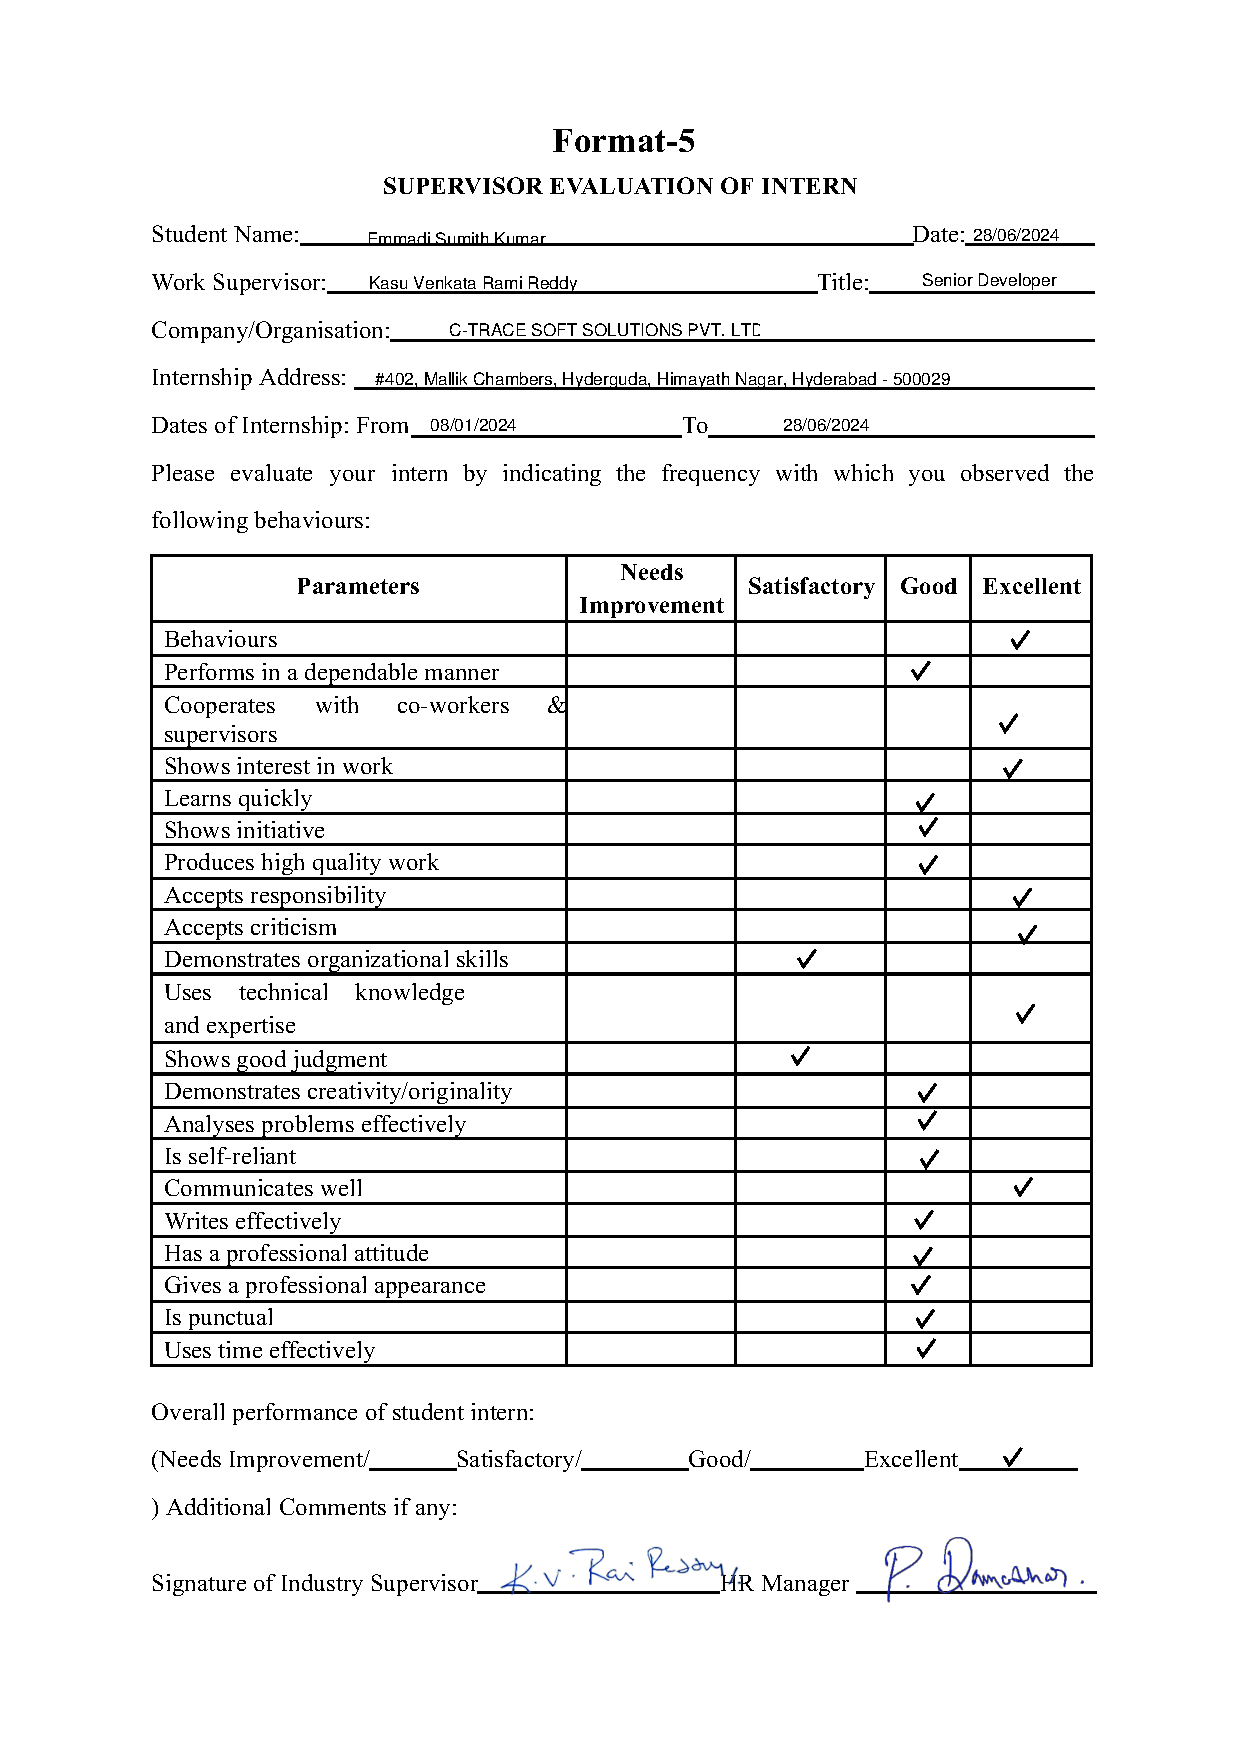
\includepdf[scale=1,pages={1},pagecommand={\thispagestyle{plain}}]{UI20CS21_Format5.pdf}
    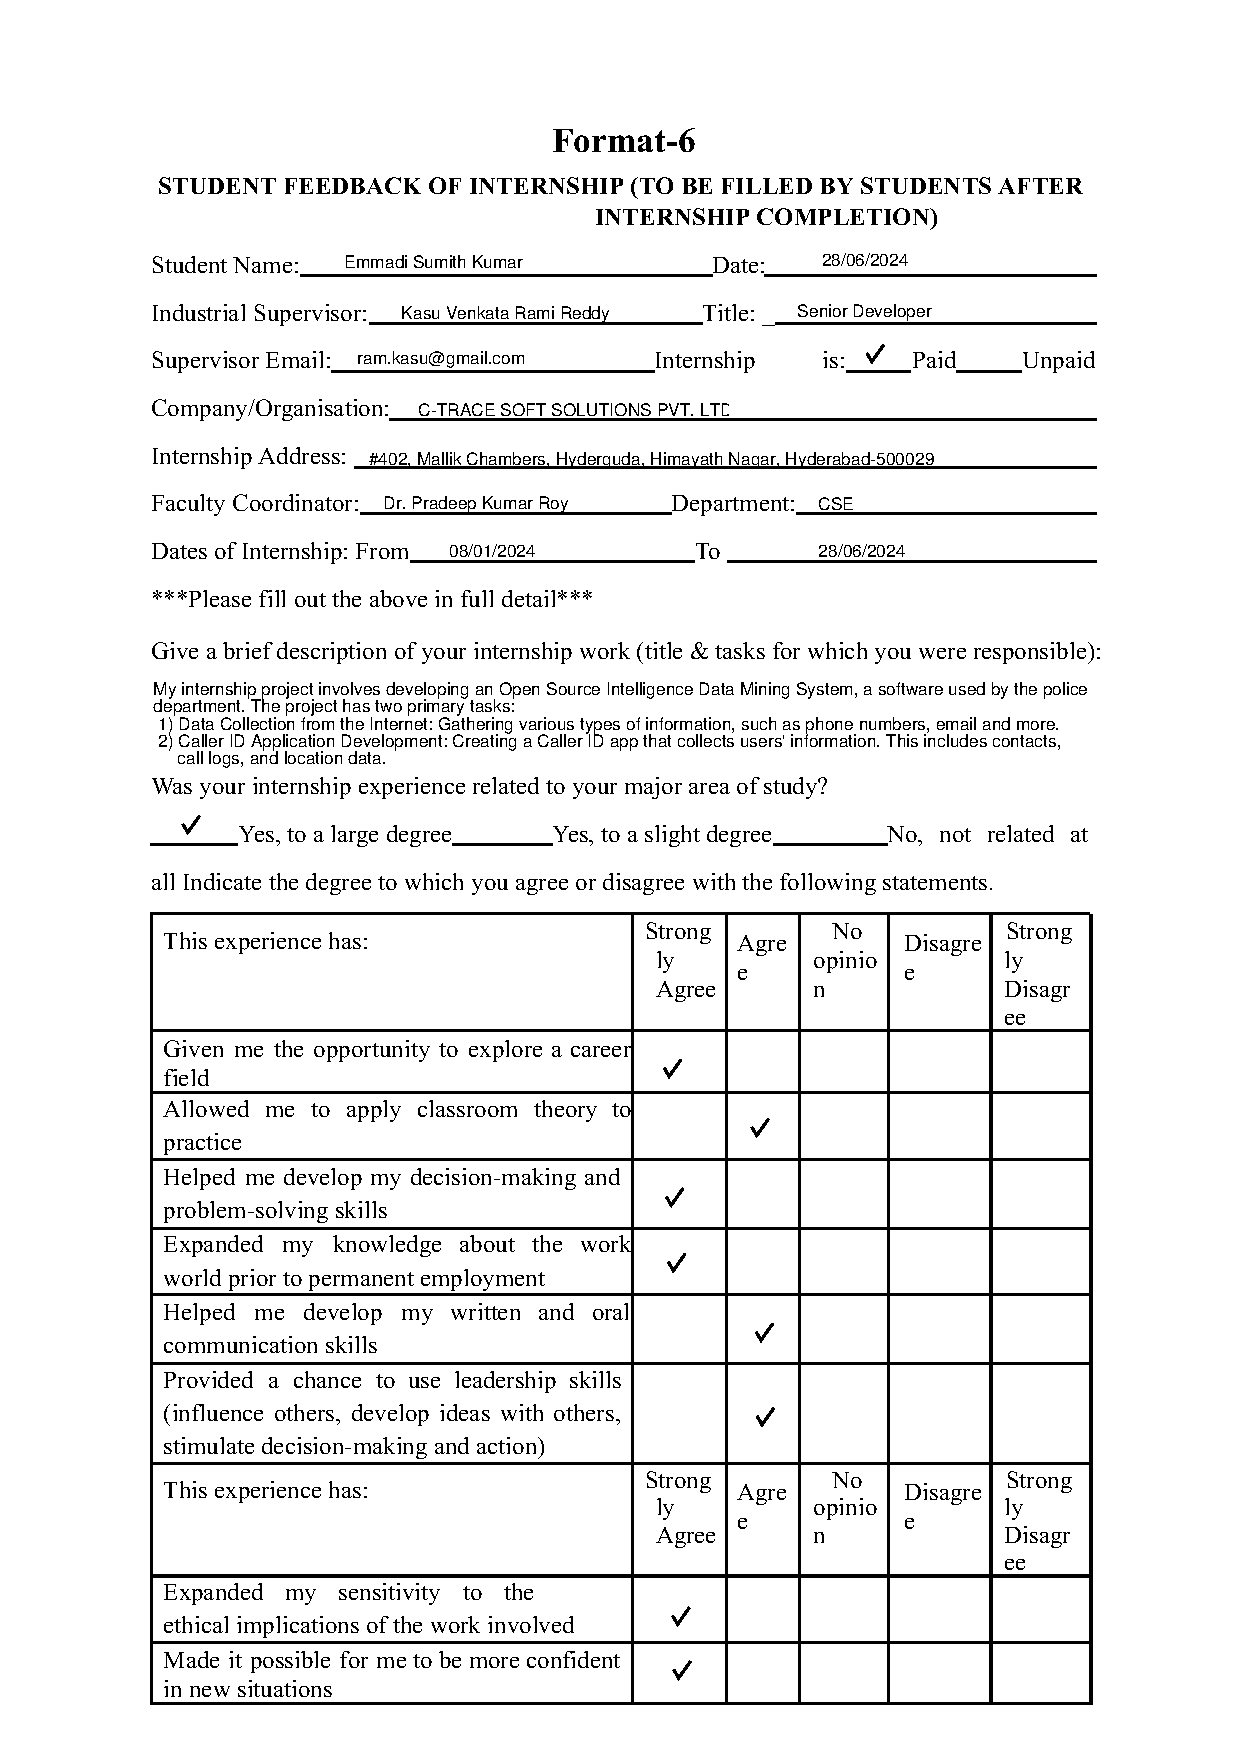
\includepdf[scale=1,pages={1,2},pagecommand={\thispagestyle{plain}}]{UI20CS21_Format6.pdf}

    \phantomsection
    \addcontentsline{toc}{chapter}{Student Feedback of Internship}
    %\includepdf[scale=1,pages={2,3}, pagecommand={\thispagestyle{plain}}]{Extras/5and6.pdf}

    \phantomsection
    \addcontentsline{toc}{chapter}{Plagiarism Report}
    %\includepdf[scale=1,pages={1}, pagecommand={\thispagestyle{plain}}]{Extras/Plagiarism.pdf}

    
    \phantomsection
    \addcontentsline{toc}{chapter}{Daily Logs}
     %\includepdf[scale=1,pages=-, pagecommand={\thispagestyle{plain}}]{Extras/Book1.pdf}
    

    % \newpage
    % \includepdf[scale=0.75,pages=-,pagecommand=\textbf{\large{APPENDIX-A: Guide}}]{Appendix/GUIDE.pdf}
    % % \setboolean{@twoside}{false}
% \newpage
% \includepdf[scale=0.8,pages=-,pagecommand=\textbf{\LARGE{APPENDIX - A}}]{Guide.pdf}

\end{document}
